\documentclass[twoside]{book}

% Packages required by doxygen
\usepackage{fixltx2e}
\usepackage{calc}
\usepackage{doxygen}
\usepackage[export]{adjustbox} % also loads graphicx
\usepackage{graphicx}
\usepackage[utf8]{inputenc}
\usepackage{makeidx}
\usepackage{multicol}
\usepackage{multirow}
\PassOptionsToPackage{warn}{textcomp}
\usepackage{textcomp}
\usepackage[nointegrals]{wasysym}
\usepackage[table]{xcolor}

% Font selection
\usepackage[T1]{fontenc}
\usepackage[scaled=.90]{helvet}
\usepackage{courier}
\usepackage{amssymb}
\usepackage{sectsty}
\renewcommand{\familydefault}{\sfdefault}
\allsectionsfont{%
  \fontseries{bc}\selectfont%
  \color{darkgray}%
}
\renewcommand{\DoxyLabelFont}{%
  \fontseries{bc}\selectfont%
  \color{darkgray}%
}
\newcommand{\+}{\discretionary{\mbox{\scriptsize$\hookleftarrow$}}{}{}}

% Page & text layout
\usepackage{geometry}
\geometry{%
  a4paper,%
  top=2.5cm,%
  bottom=2.5cm,%
  left=2.5cm,%
  right=2.5cm%
}
\tolerance=750
\hfuzz=15pt
\hbadness=750
\setlength{\emergencystretch}{15pt}
\setlength{\parindent}{0cm}
\setlength{\parskip}{3ex plus 2ex minus 2ex}
\makeatletter
\renewcommand{\paragraph}{%
  \@startsection{paragraph}{4}{0ex}{-1.0ex}{1.0ex}{%
    \normalfont\normalsize\bfseries\SS@parafont%
  }%
}
\renewcommand{\subparagraph}{%
  \@startsection{subparagraph}{5}{0ex}{-1.0ex}{1.0ex}{%
    \normalfont\normalsize\bfseries\SS@subparafont%
  }%
}
\makeatother

% Headers & footers
\usepackage{fancyhdr}
\pagestyle{fancyplain}
\fancyhead[LE]{\fancyplain{}{\bfseries\thepage}}
\fancyhead[CE]{\fancyplain{}{}}
\fancyhead[RE]{\fancyplain{}{\bfseries\leftmark}}
\fancyhead[LO]{\fancyplain{}{\bfseries\rightmark}}
\fancyhead[CO]{\fancyplain{}{}}
\fancyhead[RO]{\fancyplain{}{\bfseries\thepage}}
\fancyfoot[LE]{\fancyplain{}{}}
\fancyfoot[CE]{\fancyplain{}{}}
\fancyfoot[RE]{\fancyplain{}{\bfseries\scriptsize Generated by Doxygen }}
\fancyfoot[LO]{\fancyplain{}{\bfseries\scriptsize Generated by Doxygen }}
\fancyfoot[CO]{\fancyplain{}{}}
\fancyfoot[RO]{\fancyplain{}{}}
\renewcommand{\footrulewidth}{0.4pt}
\renewcommand{\chaptermark}[1]{%
  \markboth{#1}{}%
}
\renewcommand{\sectionmark}[1]{%
  \markright{\thesection\ #1}%
}

% Indices & bibliography
\usepackage{natbib}
\usepackage[titles]{tocloft}
\setcounter{tocdepth}{3}
\setcounter{secnumdepth}{5}
\makeindex

% Hyperlinks (required, but should be loaded last)
\usepackage{ifpdf}
\ifpdf
  \usepackage[pdftex,pagebackref=true]{hyperref}
\else
  \usepackage[ps2pdf,pagebackref=true]{hyperref}
\fi
\hypersetup{%
  colorlinks=true,%
  linkcolor=blue,%
  citecolor=blue,%
  unicode%
}

% Custom commands
\newcommand{\clearemptydoublepage}{%
  \newpage{\pagestyle{empty}\cleardoublepage}%
}

\usepackage{caption}
\captionsetup{labelsep=space,justification=centering,font={bf},singlelinecheck=off,skip=4pt,position=top}

%===== C O N T E N T S =====

\begin{document}

% Titlepage & ToC
\hypersetup{pageanchor=false,
             bookmarksnumbered=true,
             pdfencoding=unicode
            }
\pagenumbering{roman}
\begin{titlepage}
\vspace*{7cm}
\begin{center}%
{\Large Game\+Engine }\\
\vspace*{1cm}
{\large Generated by Doxygen 1.8.11}\\
\end{center}
\end{titlepage}
\clearemptydoublepage
\tableofcontents
\clearemptydoublepage
\pagenumbering{arabic}
\hypersetup{pageanchor=true}

%--- Begin generated contents ---
\chapter{Hierarchical Index}
\section{Class Hierarchy}
This inheritance list is sorted roughly, but not completely, alphabetically\+:\begin{DoxyCompactList}
\item \contentsline{section}{App\+Delegate()}{\pageref{category_app_delegate_07_08}}{}
\item $<$U\+I\+Application\+Delegate$>$\begin{DoxyCompactList}
\item \contentsline{section}{App\+Delegate}{\pageref{interface_app_delegate}}{}
\end{DoxyCompactList}
\item U\+I\+Responder\begin{DoxyCompactList}
\item \contentsline{section}{App\+Delegate}{\pageref{interface_app_delegate}}{}
\end{DoxyCompactList}
\end{DoxyCompactList}

\chapter{Class Index}
\section{Class List}
Here are the classes, structs, unions and interfaces with brief descriptions\+:\begin{DoxyCompactList}
\item\contentsline{section}{\hyperlink{interface_app_delegate}{App\+Delegate} }{\pageref{interface_app_delegate}}{}
\item\contentsline{section}{\hyperlink{category_app_delegate_07_08}{App\+Delegate()} }{\pageref{category_app_delegate_07_08}}{}
\item\contentsline{section}{\hyperlink{interface_camera}{Camera} }{\pageref{interface_camera}}{}
\item\contentsline{section}{\hyperlink{interface_cube}{Cube} }{\pageref{interface_cube}}{}
\item\contentsline{section}{\hyperlink{interface_entity}{Entity} }{\pageref{interface_entity}}{}
\item\contentsline{section}{\hyperlink{interface_entity_render}{Entity\+Render} }{\pageref{interface_entity_render}}{}
\item\contentsline{section}{\hyperlink{interface_entity_shader_manager}{Entity\+Shader\+Manager} }{\pageref{interface_entity_shader_manager}}{}
\item\contentsline{section}{\hyperlink{interface_game_engine_tests}{Game\+Engine\+Tests} }{\pageref{interface_game_engine_tests}}{}
\item\contentsline{section}{\hyperlink{interface_game_view_controller}{Game\+View\+Controller} }{\pageref{interface_game_view_controller}}{}
\item\contentsline{section}{\hyperlink{category_game_view_controller_07_08}{Game\+View\+Controller()} }{\pageref{category_game_view_controller_07_08}}{}
\item\contentsline{section}{\hyperlink{interface_g_l_s_l_utils}{G\+L\+S\+L\+Utils} }{\pageref{interface_g_l_s_l_utils}}{}
\item\contentsline{section}{\hyperlink{protocol_i_shape-p}{$<$\+I\+Shape$>$} }{\pageref{protocol_i_shape-p}}{}
\item\contentsline{section}{\hyperlink{interface_loader}{Loader} }{\pageref{interface_loader}}{}
\item\contentsline{section}{\hyperlink{interface_load_utils}{Load\+Utils} }{\pageref{interface_load_utils}}{}
\item\contentsline{section}{\hyperlink{interface_master_render}{Master\+Render} }{\pageref{interface_master_render}}{}
\item\contentsline{section}{\hyperlink{interface_model_texture}{Model\+Texture} }{\pageref{interface_model_texture}}{}
\item\contentsline{section}{\hyperlink{interface_raw_model}{Raw\+Model} }{\pageref{interface_raw_model}}{}
\item\contentsline{section}{\hyperlink{interface_shader_manager}{Shader\+Manager} }{\pageref{interface_shader_manager}}{}
\item\contentsline{section}{\hyperlink{interface_shader_program}{Shader\+Program} }{\pageref{interface_shader_program}}{}
\item\contentsline{section}{\hyperlink{interface_sky_box}{Sky\+Box} }{\pageref{interface_sky_box}}{}
\item\contentsline{section}{\hyperlink{interface_sky_box_shape}{Sky\+Box\+Shape} }{\pageref{interface_sky_box_shape}}{}
\item\contentsline{section}{\hyperlink{interface_terrain}{Terrain} }{\pageref{interface_terrain}}{}
\item\contentsline{section}{\hyperlink{interface_terrain_shape}{Terrain\+Shape} }{\pageref{interface_terrain_shape}}{}
\item\contentsline{section}{\hyperlink{interface_terrain_textures_pack}{Terrain\+Textures\+Pack} }{\pageref{interface_terrain_textures_pack}}{}
\item\contentsline{section}{\hyperlink{interface_textured_model}{Textured\+Model} }{\pageref{interface_textured_model}}{}
\item\contentsline{section}{\hyperlink{interface_vector2f}{Vector2f} }{\pageref{interface_vector2f}}{}
\item\contentsline{section}{\hyperlink{interface_vector3f}{Vector3f} }{\pageref{interface_vector3f}}{}
\end{DoxyCompactList}

\chapter{Class Documentation}
\hypertarget{interface_app_delegate}{}\section{App\+Delegate Class Reference}
\label{interface_app_delegate}\index{App\+Delegate@{App\+Delegate}}
Inheritance diagram for App\+Delegate\+:\begin{figure}[H]
\begin{center}
\leavevmode
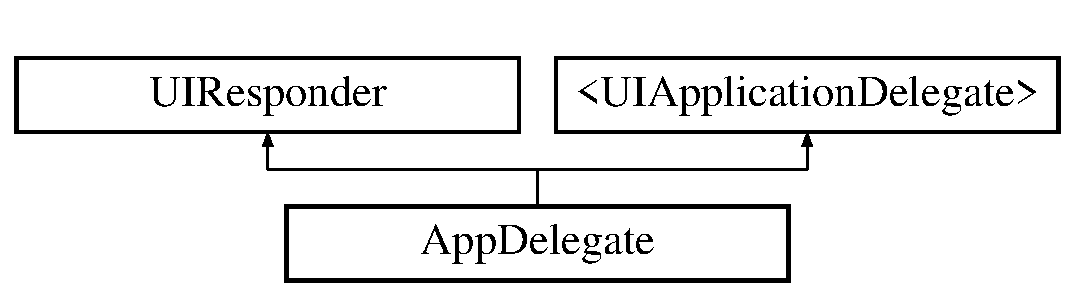
\includegraphics[height=2.000000cm]{interface_app_delegate}
\end{center}
\end{figure}
\subsection*{Properties}
\begin{DoxyCompactItemize}
\item 
U\+I\+Window $\ast$ {\bfseries window}\hypertarget{interface_app_delegate_acf48ac24125e688cac1a85445cd7fac2}{}\label{interface_app_delegate_acf48ac24125e688cac1a85445cd7fac2}

\end{DoxyCompactItemize}


The documentation for this class was generated from the following file\+:\begin{DoxyCompactItemize}
\item 
Game\+Engine/App\+Delegate.\+h\end{DoxyCompactItemize}

\hypertarget{category_app_delegate_07_08}{}\section{App\+Delegate() Category Reference}
\label{category_app_delegate_07_08}\index{App\+Delegate()@{App\+Delegate()}}


The documentation for this category was generated from the following file\+:\begin{DoxyCompactItemize}
\item 
Game\+Engine/App\+Delegate.\+m\end{DoxyCompactItemize}

\hypertarget{interface_camera}{}\section{Camera Class Reference}
\label{interface_camera}\index{Camera@{Camera}}


{\ttfamily \#import $<$Camera.\+h$>$}

Inheritance diagram for Camera\+:\begin{figure}[H]
\begin{center}
\leavevmode
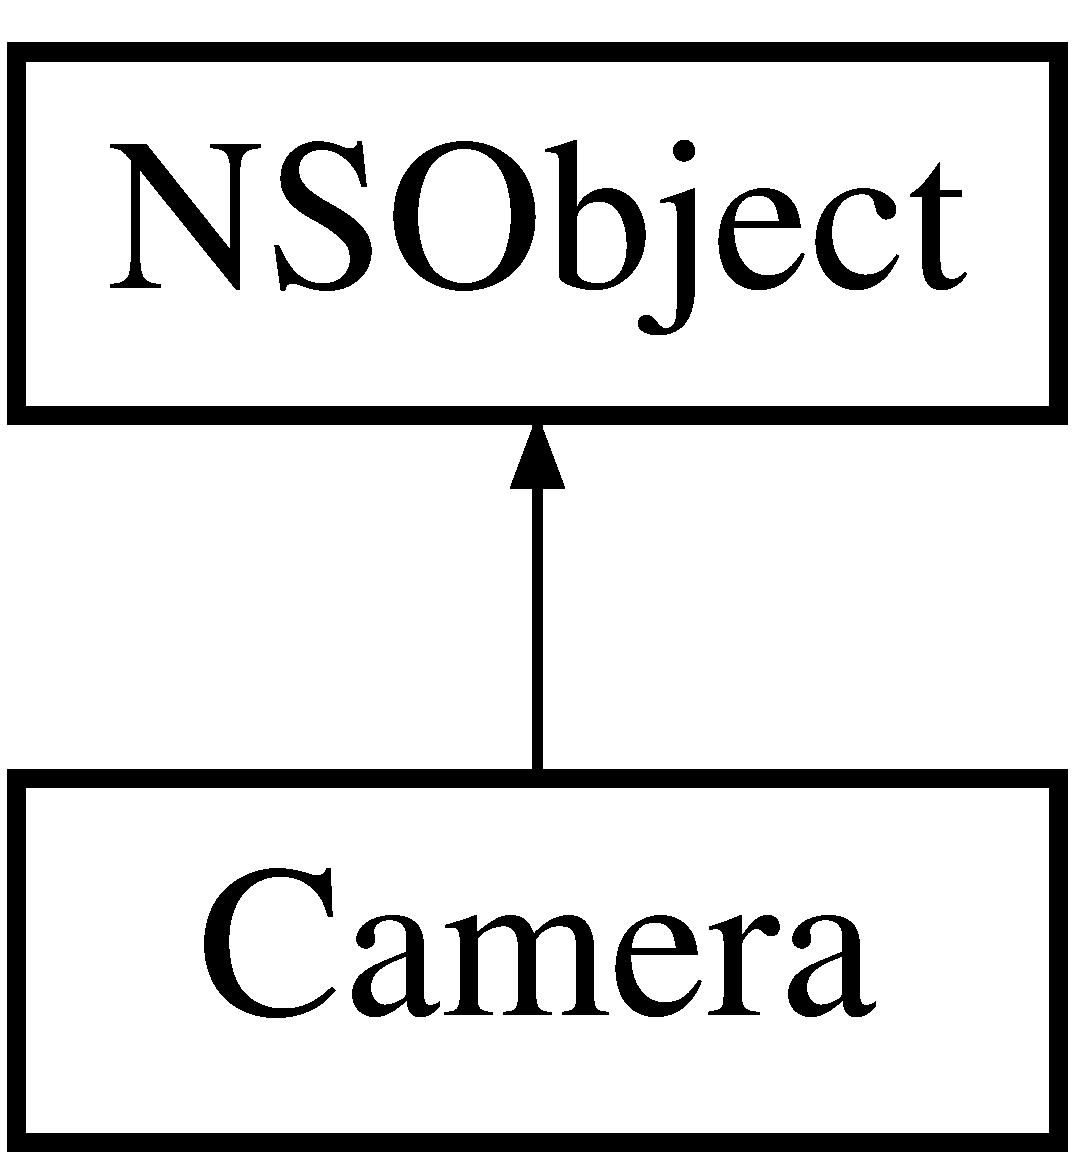
\includegraphics[height=2.000000cm]{interface_camera}
\end{center}
\end{figure}
\subsection*{Instance Methods}
\begin{DoxyCompactItemize}
\item 
(id) -\/ \hyperlink{interface_camera_a4633f7c2d8c298e9162d5c5b6a6ffe2c}{init}
\item 
(void) -\/ \hyperlink{interface_camera_a8414e6d74d3f6259fa5ea1f037e9d8bd}{move}
\item 
(void) -\/ \hyperlink{interface_camera_a89225863307bdbd309fb52a7904bc4db}{rotate}
\end{DoxyCompactItemize}
\subsection*{Properties}
\begin{DoxyCompactItemize}
\item 
\hyperlink{interface_vector3f}{Vector3f} $\ast$ \hyperlink{interface_camera_a59764f8faf1cd481eaa02d504ed088cd}{position}
\item 
float \hyperlink{interface_camera_ab56fcb39f580e8d2159cf2c9c6d9a65a}{pitch}
\item 
float \hyperlink{interface_camera_ad76701b22630f2df28a0ae15f0497a3a}{yaw}
\item 
float \hyperlink{interface_camera_a08d9c6119a859e664d74ca07db4fe3d3}{roll}
\end{DoxyCompactItemize}


\subsection{Detailed Description}
Represents the the camera used by the user to see the 3D World 

\subsection{Method Documentation}
\index{Camera@{Camera}!init@{init}}
\index{init@{init}!Camera@{Camera}}
\subsubsection[{\texorpdfstring{init()}{init()}}]{\setlength{\rightskip}{0pt plus 5cm}-\/ (id) init 
\begin{DoxyParamCaption}
{}
\end{DoxyParamCaption}
}\hypertarget{interface_camera_a4633f7c2d8c298e9162d5c5b6a6ffe2c}{}\label{interface_camera_a4633f7c2d8c298e9162d5c5b6a6ffe2c}
Initiator of camera \index{Camera@{Camera}!move@{move}}
\index{move@{move}!Camera@{Camera}}
\subsubsection[{\texorpdfstring{move()}{move()}}]{\setlength{\rightskip}{0pt plus 5cm}-\/ (void) move 
\begin{DoxyParamCaption}
{}
\end{DoxyParamCaption}
}\hypertarget{interface_camera_a8414e6d74d3f6259fa5ea1f037e9d8bd}{}\label{interface_camera_a8414e6d74d3f6259fa5ea1f037e9d8bd}
Read the keys pressed by the used and updates the position of the camera \index{Camera@{Camera}!rotate@{rotate}}
\index{rotate@{rotate}!Camera@{Camera}}
\subsubsection[{\texorpdfstring{rotate()}{rotate()}}]{\setlength{\rightskip}{0pt plus 5cm}-\/ (void) rotate 
\begin{DoxyParamCaption}
{}
\end{DoxyParamCaption}
}\hypertarget{interface_camera_a89225863307bdbd309fb52a7904bc4db}{}\label{interface_camera_a89225863307bdbd309fb52a7904bc4db}
Rotate the camera that the user sees 

\subsection{Property Documentation}
\index{Camera@{Camera}!pitch@{pitch}}
\index{pitch@{pitch}!Camera@{Camera}}
\subsubsection[{\texorpdfstring{pitch}{pitch}}]{\setlength{\rightskip}{0pt plus 5cm}-\/ (float) pitch\hspace{0.3cm}{\ttfamily [read]}, {\ttfamily [atomic]}, {\ttfamily [assign]}}\hypertarget{interface_camera_ab56fcb39f580e8d2159cf2c9c6d9a65a}{}\label{interface_camera_ab56fcb39f580e8d2159cf2c9c6d9a65a}
Pitch is up and down (rotation around X-\/axis) \index{Camera@{Camera}!position@{position}}
\index{position@{position}!Camera@{Camera}}
\subsubsection[{\texorpdfstring{position}{position}}]{\setlength{\rightskip}{0pt plus 5cm}-\/ ({\bf Vector3f}$\ast$) position\hspace{0.3cm}{\ttfamily [read]}, {\ttfamily [atomic]}, {\ttfamily [assign]}}\hypertarget{interface_camera_a59764f8faf1cd481eaa02d504ed088cd}{}\label{interface_camera_a59764f8faf1cd481eaa02d504ed088cd}
The position where the camera is \index{Camera@{Camera}!roll@{roll}}
\index{roll@{roll}!Camera@{Camera}}
\subsubsection[{\texorpdfstring{roll}{roll}}]{\setlength{\rightskip}{0pt plus 5cm}-\/ (float) roll\hspace{0.3cm}{\ttfamily [read]}, {\ttfamily [atomic]}, {\ttfamily [assign]}}\hypertarget{interface_camera_a08d9c6119a859e664d74ca07db4fe3d3}{}\label{interface_camera_a08d9c6119a859e664d74ca07db4fe3d3}
Roll, which we usually don\textquotesingle{}t experience is when you tilt your head (rotation around Z-\/axis) \index{Camera@{Camera}!yaw@{yaw}}
\index{yaw@{yaw}!Camera@{Camera}}
\subsubsection[{\texorpdfstring{yaw}{yaw}}]{\setlength{\rightskip}{0pt plus 5cm}-\/ (float) yaw\hspace{0.3cm}{\ttfamily [read]}, {\ttfamily [atomic]}, {\ttfamily [assign]}}\hypertarget{interface_camera_ad76701b22630f2df28a0ae15f0497a3a}{}\label{interface_camera_ad76701b22630f2df28a0ae15f0497a3a}
Yaw is the angle when moving the head left and right (rotation around Y-\/axis) 

The documentation for this class was generated from the following files\+:\begin{DoxyCompactItemize}
\item 
Game\+Engine/\+Models/Camera.\+h\item 
Game\+Engine/\+Models/Camera.\+m\end{DoxyCompactItemize}

\hypertarget{interface_cube}{}\section{Cube Class Reference}
\label{interface_cube}\index{Cube@{Cube}}
Inheritance diagram for Cube\+:\begin{figure}[H]
\begin{center}
\leavevmode
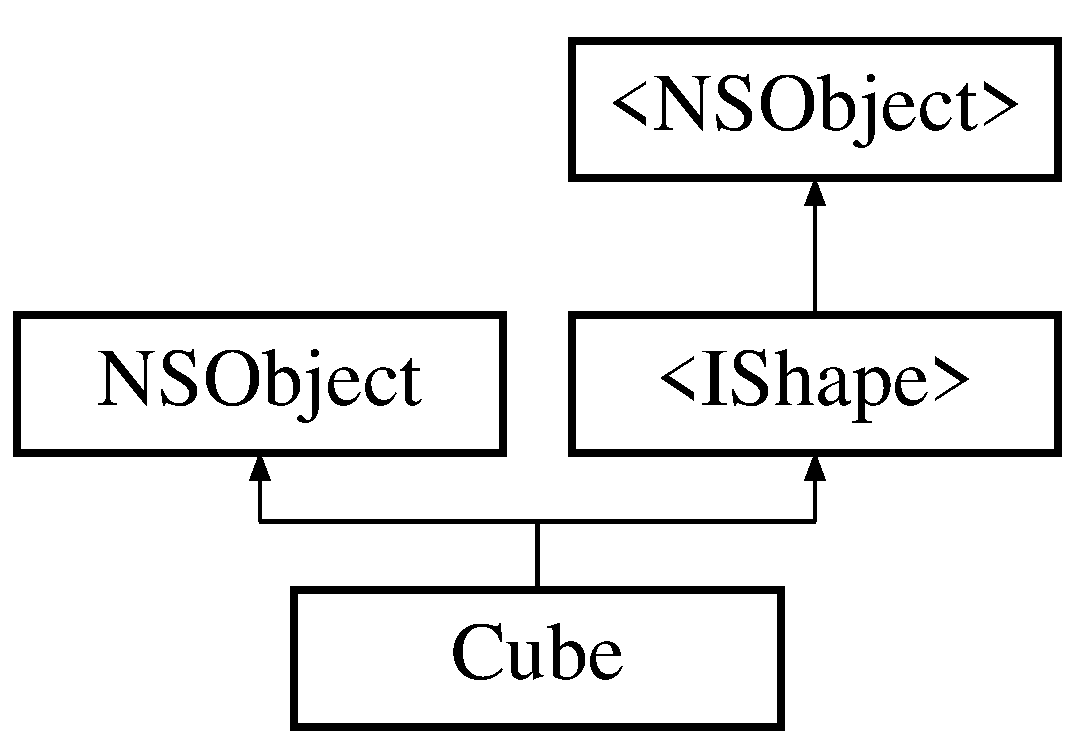
\includegraphics[height=3.000000cm]{interface_cube}
\end{center}
\end{figure}
\subsection*{Additional Inherited Members}


The documentation for this class was generated from the following file\+:\begin{DoxyCompactItemize}
\item 
Game\+Engine/\+Shapes/Cube.\+h\end{DoxyCompactItemize}

\hypertarget{interface_entity}{}\section{Entity Class Reference}
\label{interface_entity}\index{Entity@{Entity}}


{\ttfamily \#import $<$Entity.\+h$>$}

Inheritance diagram for Entity\+:\begin{figure}[H]
\begin{center}
\leavevmode
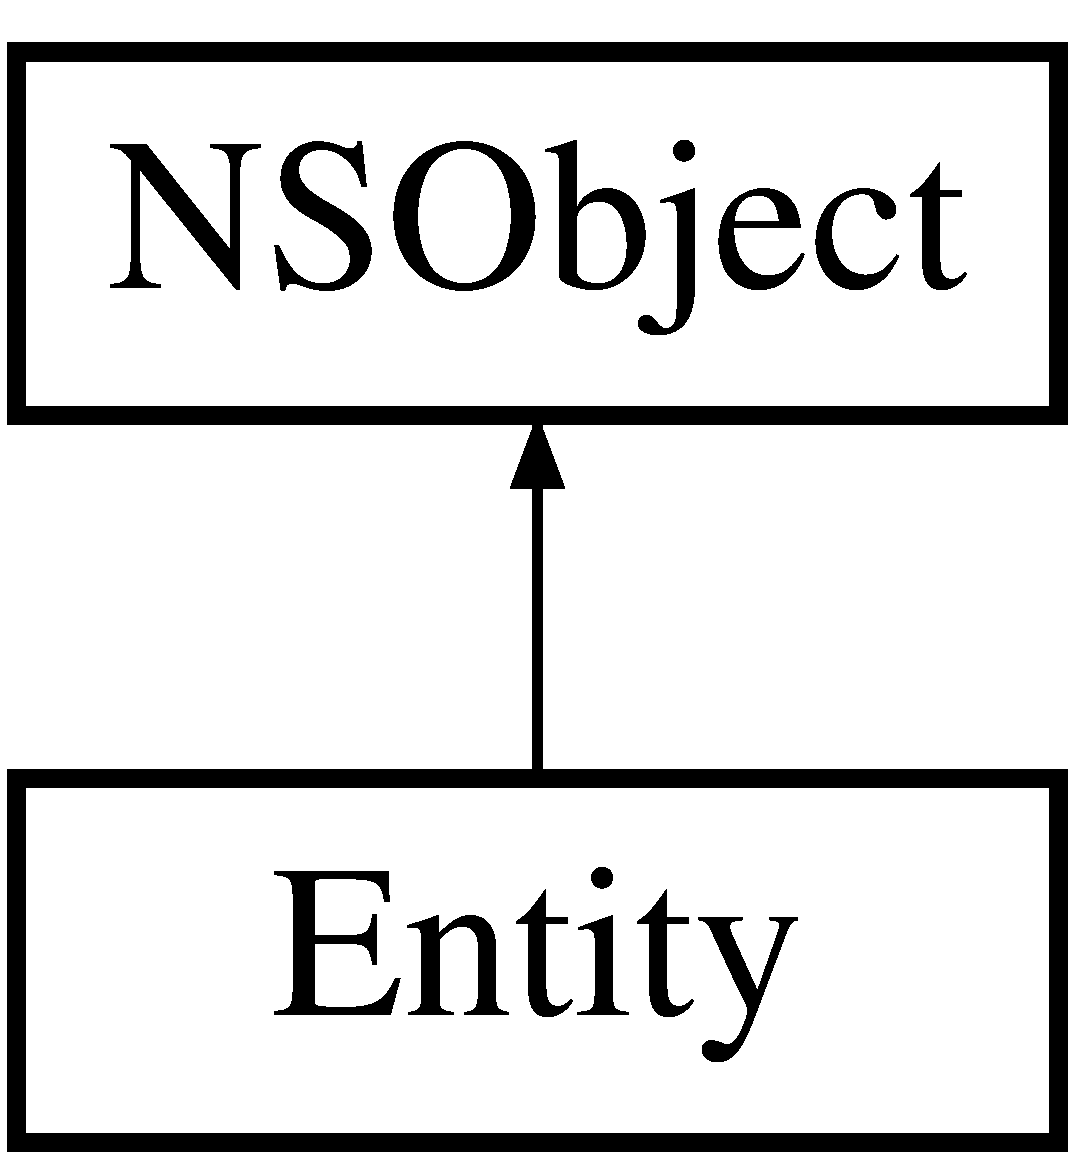
\includegraphics[height=2.000000cm]{interface_entity}
\end{center}
\end{figure}
\subsection*{Instance Methods}
\begin{DoxyCompactItemize}
\item 
(id) -\/ \hyperlink{interface_entity_ad7147d00332fed30cf14829243c5430e}{init\+::::::}
\item 
(void) -\/ \hyperlink{interface_entity_a51ba5b8f3b66cba0b722edaabdd6090e}{increase\+Position\+:::}
\item 
(void) -\/ \hyperlink{interface_entity_a6e21b02ee042d70378d336fe6ea16fb5}{increase\+Rotation\+:::}
\end{DoxyCompactItemize}
\subsection*{Properties}
\begin{DoxyCompactItemize}
\item 
\hyperlink{interface_textured_model}{Textured\+Model} $\ast$ {\bfseries model}\hypertarget{interface_entity_a02801075948569b0e2b52bed0e0f7c4c}{}\label{interface_entity_a02801075948569b0e2b52bed0e0f7c4c}

\item 
\hyperlink{interface_vector3f}{Vector3f} $\ast$ {\bfseries position}\hypertarget{interface_entity_a5b46de87209b8b087852e4cd92e4218c}{}\label{interface_entity_a5b46de87209b8b087852e4cd92e4218c}

\item 
float {\bfseries rotX}\hypertarget{interface_entity_a872123c5ed32f888d9d34114fcded890}{}\label{interface_entity_a872123c5ed32f888d9d34114fcded890}

\item 
float {\bfseries rotY}\hypertarget{interface_entity_ab786b45308be8e93648e092703910909}{}\label{interface_entity_ab786b45308be8e93648e092703910909}

\item 
float {\bfseries rotZ}\hypertarget{interface_entity_aea2a72cc52774873d440d6098b4adfe7}{}\label{interface_entity_aea2a72cc52774873d440d6098b4adfe7}

\item 
float {\bfseries scale}\hypertarget{interface_entity_a8c1b0331fdaca5874c15e10de1ed3531}{}\label{interface_entity_a8c1b0331fdaca5874c15e10de1ed3531}

\end{DoxyCompactItemize}


\subsection{Detailed Description}
Represents one entity in the 3D world 

\subsection{Method Documentation}
\index{Entity@{Entity}!increase\+Position\+:::@{increase\+Position\+:::}}
\index{increase\+Position\+:::@{increase\+Position\+:::}!Entity@{Entity}}
\subsubsection[{\texorpdfstring{increase\+Position\+:::(float dx,[] float dy,[] float dz)}{increasePosition:::(float dx,[] float dy,[] float dz)}}]{\setlength{\rightskip}{0pt plus 5cm}-\/ (void) increase\+Position\+: 
\begin{DoxyParamCaption}
\item[{(float)}]{dx}
\item[{:(float)}]{dy}
\item[{:(float)}]{dz}
\end{DoxyParamCaption}
}\hypertarget{interface_entity_a51ba5b8f3b66cba0b722edaabdd6090e}{}\label{interface_entity_a51ba5b8f3b66cba0b722edaabdd6090e}
Increases the position of the model using for that the specified components


\begin{DoxyParams}{Parameters}
{\em dx} & X component to be increase \\
\hline
{\em dy} & Y component to be increase \\
\hline
{\em dz} & Z component to be increase \\
\hline
\end{DoxyParams}
\index{Entity@{Entity}!increase\+Rotation\+:::@{increase\+Rotation\+:::}}
\index{increase\+Rotation\+:::@{increase\+Rotation\+:::}!Entity@{Entity}}
\subsubsection[{\texorpdfstring{increase\+Rotation\+:::(float dx,[] float dy,[] float dz)}{increaseRotation:::(float dx,[] float dy,[] float dz)}}]{\setlength{\rightskip}{0pt plus 5cm}-\/ (void) increase\+Rotation\+: 
\begin{DoxyParamCaption}
\item[{(float)}]{dx}
\item[{:(float)}]{dy}
\item[{:(float)}]{dz}
\end{DoxyParamCaption}
}\hypertarget{interface_entity_a6e21b02ee042d70378d336fe6ea16fb5}{}\label{interface_entity_a6e21b02ee042d70378d336fe6ea16fb5}
Increases the rotation of the model using for that the specified components 
\begin{DoxyParams}{Parameters}
{\em dx} & X component to be increase \\
\hline
{\em dy} & Y component to be increase \\
\hline
{\em dz} & Z component to be increase \\
\hline
\end{DoxyParams}
\index{Entity@{Entity}!init\+::::::@{init\+::::::}}
\index{init\+::::::@{init\+::::::}!Entity@{Entity}}
\subsubsection[{\texorpdfstring{init\+::::::(\+Textured\+Model $\ast$a\+Model,[] Vector3f $\ast$a\+Position,[] float a\+Rot\+X,[] float a\+Rot\+Y,[] float a\+Rot\+Z,[] float a\+Scale)}{init::::::(TexturedModel *aModel,[] Vector3f *aPosition,[] float aRotX,[] float aRotY,[] float aRotZ,[] float aScale)}}]{\setlength{\rightskip}{0pt plus 5cm}-\/ (id) init\+: 
\begin{DoxyParamCaption}
\item[{({\bf Textured\+Model}$\ast$)}]{a\+Model}
\item[{:({\bf Vector3f}$\ast$)}]{a\+Position}
\item[{:(float)}]{a\+RotX}
\item[{:(float)}]{a\+RotY}
\item[{:(float)}]{a\+RotZ}
\item[{:(float)}]{a\+Scale}
\end{DoxyParamCaption}
}\hypertarget{interface_entity_ad7147d00332fed30cf14829243c5430e}{}\label{interface_entity_ad7147d00332fed30cf14829243c5430e}
Initiator of the entity to be render in the 3D world


\begin{DoxyParams}{Parameters}
{\em a\+Model} & Textured model \\
\hline
{\em a\+Position} & Position where the model should be render \\
\hline
{\em a\+RotX} & Rotation of the model in the X axle \\
\hline
{\em a\+RotY} & Rotation of the model in the Y axle \\
\hline
{\em a\+RotZ} & Rotation of the model in the Z axle \\
\hline
{\em a\+Scale} & Scale of the model\\
\hline
\end{DoxyParams}
Initiator of the entity to be render in the 3D world


\begin{DoxyParams}{Parameters}
{\em a\+Model} & Textured model \\
\hline
{\em position} & Position where the model should be render \\
\hline
{\em a\+RotX} & Rotation of the model in the X axle \\
\hline
{\em a\+RotY} & Rotation of the model in the Y axle \\
\hline
{\em a\+RotZ} & Rotation of the model in the Z axle \\
\hline
{\em a\+Scale} & Scale of the model \\
\hline
\end{DoxyParams}


The documentation for this class was generated from the following files\+:\begin{DoxyCompactItemize}
\item 
Game\+Engine/\+Models/Entity.\+h\item 
Game\+Engine/\+Models/Entity.\+m\end{DoxyCompactItemize}

\hypertarget{interface_entity_render}{}\section{Entity\+Render Class Reference}
\label{interface_entity_render}\index{Entity\+Render@{Entity\+Render}}
Inheritance diagram for Entity\+Render\+:\begin{figure}[H]
\begin{center}
\leavevmode
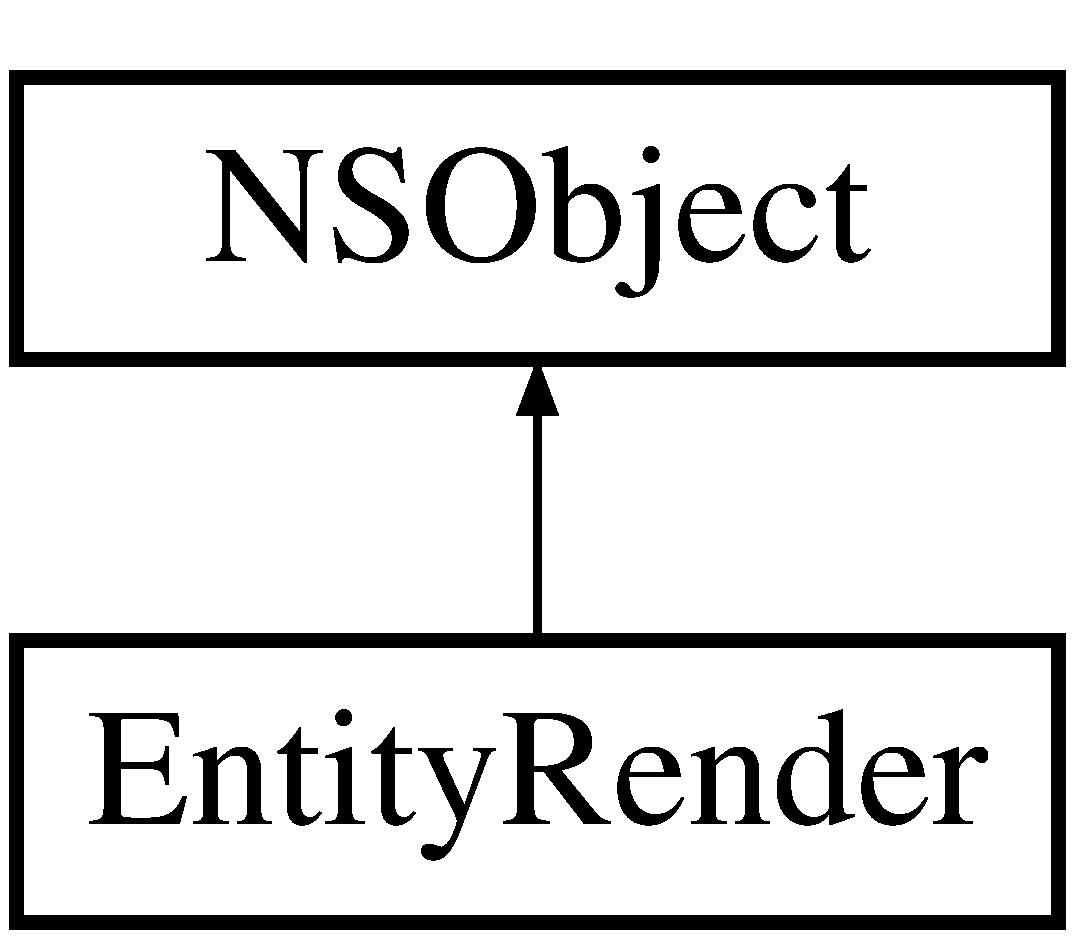
\includegraphics[height=2.000000cm]{interface_entity_render}
\end{center}
\end{figure}
\subsection*{Instance Methods}
\begin{DoxyCompactItemize}
\item 
(id) -\/ \hyperlink{interface_entity_render_a854c250e41a1f8e91421b3a1c23e4a9f}{init\+::}
\item 
(void) -\/ \hyperlink{interface_entity_render_a37c77a02d2f6f9312dbbd2db2c7585cc}{render\+:}
\end{DoxyCompactItemize}


\subsection{Detailed Description}
Class responsible to render the entities in the screen 

\subsection{Method Documentation}
\index{Entity\+Render@{Entity\+Render}!init\+::@{init\+::}}
\index{init\+::@{init\+::}!Entity\+Render@{Entity\+Render}}
\subsubsection[{\texorpdfstring{init\+::(\+Entity\+Shader\+Manager $\ast$a\+Shader,[] G\+L\+K\+Matrix4 projection\+Matrix)}{init::(EntityShaderManager *aShader,[] GLKMatrix4 projectionMatrix)}}]{\setlength{\rightskip}{0pt plus 5cm}-\/ (id) init\+: 
\begin{DoxyParamCaption}
\item[{({\bf Entity\+Shader\+Manager}$\ast$)}]{a\+Shader}
\item[{:(G\+L\+K\+Matrix4)}]{projection\+Matrix}
\end{DoxyParamCaption}
}\hypertarget{interface_entity_render_a854c250e41a1f8e91421b3a1c23e4a9f}{}\label{interface_entity_render_a854c250e41a1f8e91421b3a1c23e4a9f}
{\bfseries Initial value\+:}
\begin{DoxyCode}
\{
\textcolor{keyword}{@private}
    
    
    \hyperlink{interface_entity_shader_manager}{EntityShaderManager} *eShader
\end{DoxyCode}
Initializer of the entity render


\begin{DoxyParams}{Parameters}
{\em e\+Shader} & Shader manager \\
\hline
{\em projection\+Matrix} & The projection matrix of the render \\
\hline
\end{DoxyParams}
\index{Entity\+Render@{Entity\+Render}!render\+:@{render\+:}}
\index{render\+:@{render\+:}!Entity\+Render@{Entity\+Render}}
\subsubsection[{\texorpdfstring{render\+:(\+G\+L\+K\+Matrix4 modelview\+Matrix)}{render:(GLKMatrix4 modelviewMatrix)}}]{\setlength{\rightskip}{0pt plus 5cm}-\/ (void) render\+: 
\begin{DoxyParamCaption}
\item[{(G\+L\+K\+Matrix4)}]{modelview\+Matrix}
\end{DoxyParamCaption}
}\hypertarget{interface_entity_render_a37c77a02d2f6f9312dbbd2db2c7585cc}{}\label{interface_entity_render_a37c77a02d2f6f9312dbbd2db2c7585cc}
Render the entities in the scene


\begin{DoxyParams}{Parameters}
{\em sun} & The source of light of the scene \\
\hline
{\em view\+Matrix} & View matrix to render the scene \\
\hline
{\em entities} & List of entities of the scene \\
\hline
\end{DoxyParams}


The documentation for this class was generated from the following files\+:\begin{DoxyCompactItemize}
\item 
Game\+Engine/\+Render\+Engine/Entity\+Render.\+h\item 
Game\+Engine/\+Render\+Engine/Entity\+Render.\+m\end{DoxyCompactItemize}

\hypertarget{interface_entity_shader_manager}{}\section{Entity\+Shader\+Manager Class Reference}
\label{interface_entity_shader_manager}\index{Entity\+Shader\+Manager@{Entity\+Shader\+Manager}}
Inheritance diagram for Entity\+Shader\+Manager\+:\begin{figure}[H]
\begin{center}
\leavevmode
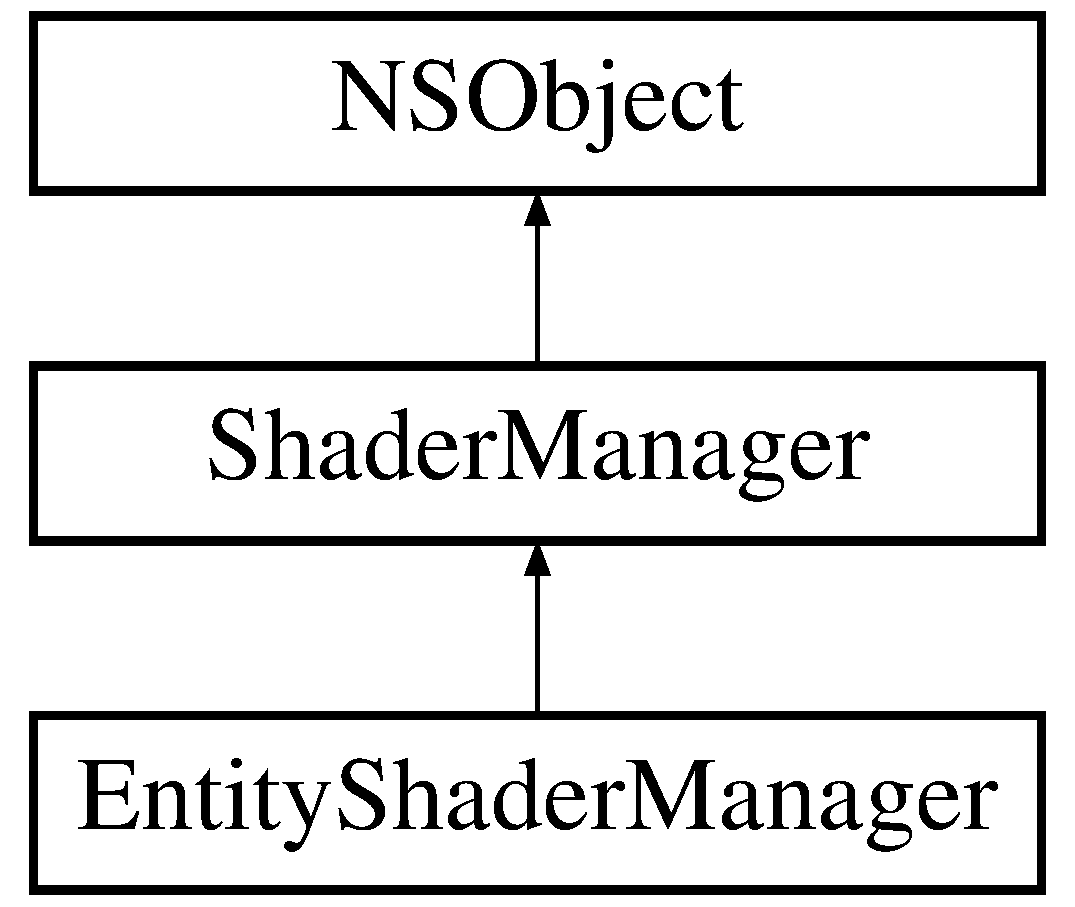
\includegraphics[height=3.000000cm]{interface_entity_shader_manager}
\end{center}
\end{figure}
\subsection*{Instance Methods}
\begin{DoxyCompactItemize}
\item 
(void) -\/ \hyperlink{interface_entity_shader_manager_aee7054ec48fb92a0136a44c6b6da287b}{load\+Projection\+Matrix\+:}
\item 
(void) -\/ \hyperlink{interface_entity_shader_manager_ab87d7a1c9557859622b5b6f0173bf9c8}{load\+View\+Matrix\+:}
\item 
(void) -\/ \hyperlink{interface_entity_shader_manager_add47708609189faa500b818c60eff323}{load\+Transformation\+Matrix\+:}
\item 
(void) -\/ {\bfseries load\+Normal\+Matrix\+:}\hypertarget{interface_entity_shader_manager_a866b613282a2edc3e3416fd89163fbd8}{}\label{interface_entity_shader_manager_a866b613282a2edc3e3416fd89163fbd8}

\end{DoxyCompactItemize}


\subsection{Detailed Description}
Manager of the shader files that are going to be load to render the 3D 

\subsection{Method Documentation}
\index{Entity\+Shader\+Manager@{Entity\+Shader\+Manager}!load\+Projection\+Matrix\+:@{load\+Projection\+Matrix\+:}}
\index{load\+Projection\+Matrix\+:@{load\+Projection\+Matrix\+:}!Entity\+Shader\+Manager@{Entity\+Shader\+Manager}}
\subsubsection[{\texorpdfstring{load\+Projection\+Matrix\+:(\+G\+L\+K\+Matrix4 matrix)}{loadProjectionMatrix:(GLKMatrix4 matrix)}}]{\setlength{\rightskip}{0pt plus 5cm}-\/ (void) load\+Projection\+Matrix\+: 
\begin{DoxyParamCaption}
\item[{(G\+L\+K\+Matrix4)}]{matrix}
\end{DoxyParamCaption}
}\hypertarget{interface_entity_shader_manager_aee7054ec48fb92a0136a44c6b6da287b}{}\label{interface_entity_shader_manager_aee7054ec48fb92a0136a44c6b6da287b}
Load the projection matrix


\begin{DoxyParams}{Parameters}
{\em matrix} & the matrix to be loaded \\
\hline
\end{DoxyParams}
\index{Entity\+Shader\+Manager@{Entity\+Shader\+Manager}!load\+Transformation\+Matrix\+:@{load\+Transformation\+Matrix\+:}}
\index{load\+Transformation\+Matrix\+:@{load\+Transformation\+Matrix\+:}!Entity\+Shader\+Manager@{Entity\+Shader\+Manager}}
\subsubsection[{\texorpdfstring{load\+Transformation\+Matrix\+:(\+G\+L\+K\+Matrix4 matrix)}{loadTransformationMatrix:(GLKMatrix4 matrix)}}]{\setlength{\rightskip}{0pt plus 5cm}-\/ (void) load\+Transformation\+Matrix\+: 
\begin{DoxyParamCaption}
\item[{(G\+L\+K\+Matrix4)}]{matrix}
\end{DoxyParamCaption}
}\hypertarget{interface_entity_shader_manager_add47708609189faa500b818c60eff323}{}\label{interface_entity_shader_manager_add47708609189faa500b818c60eff323}
Load the transformation matrix


\begin{DoxyParams}{Parameters}
{\em matrix} & the matrix to be loaded \\
\hline
\end{DoxyParams}
\index{Entity\+Shader\+Manager@{Entity\+Shader\+Manager}!load\+View\+Matrix\+:@{load\+View\+Matrix\+:}}
\index{load\+View\+Matrix\+:@{load\+View\+Matrix\+:}!Entity\+Shader\+Manager@{Entity\+Shader\+Manager}}
\subsubsection[{\texorpdfstring{load\+View\+Matrix\+:(\+G\+L\+K\+Matrix4 matrix)}{loadViewMatrix:(GLKMatrix4 matrix)}}]{\setlength{\rightskip}{0pt plus 5cm}-\/ (void) load\+View\+Matrix\+: 
\begin{DoxyParamCaption}
\item[{(G\+L\+K\+Matrix4)}]{matrix}
\end{DoxyParamCaption}
}\hypertarget{interface_entity_shader_manager_ab87d7a1c9557859622b5b6f0173bf9c8}{}\label{interface_entity_shader_manager_ab87d7a1c9557859622b5b6f0173bf9c8}
Load the view matrix


\begin{DoxyParams}{Parameters}
{\em matrix} & the matrix to be loaded \\
\hline
\end{DoxyParams}


The documentation for this class was generated from the following files\+:\begin{DoxyCompactItemize}
\item 
Game\+Engine/\+Shaders/\+Entities/Entity\+Shader\+Manager.\+h\item 
Game\+Engine/\+Shaders/\+Entities/Entity\+Shader\+Manager.\+m\end{DoxyCompactItemize}

\hypertarget{interface_game_engine_tests}{}\section{Game\+Engine\+Tests Class Reference}
\label{interface_game_engine_tests}\index{Game\+Engine\+Tests@{Game\+Engine\+Tests}}
Inheritance diagram for Game\+Engine\+Tests\+:\begin{figure}[H]
\begin{center}
\leavevmode
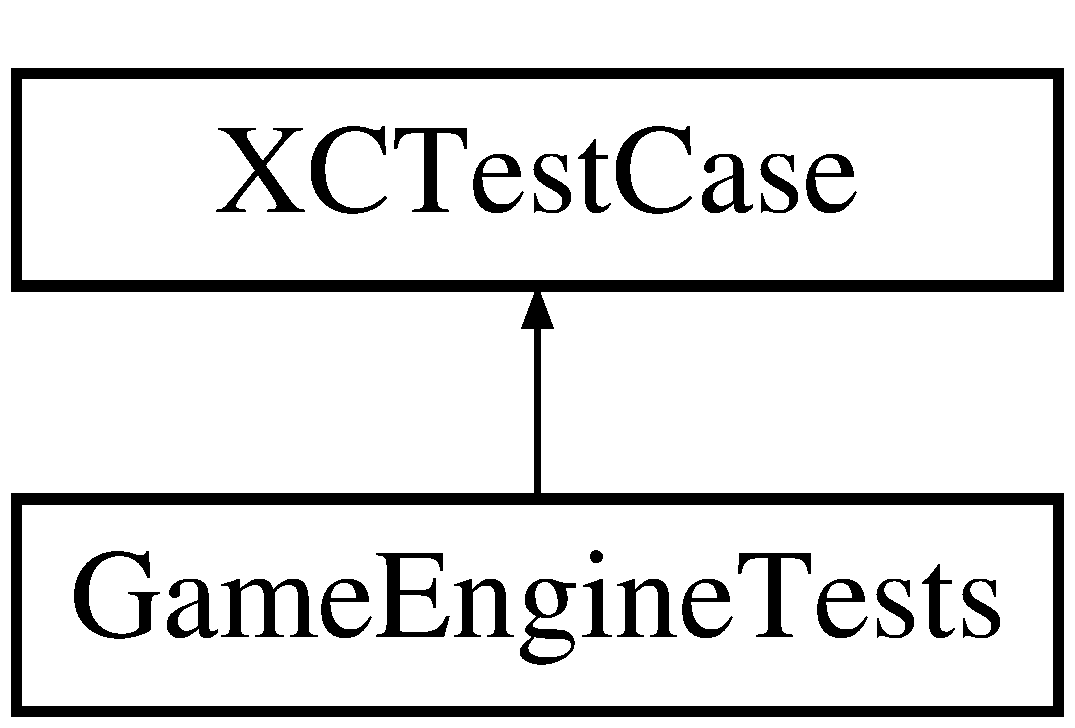
\includegraphics[height=2.000000cm]{interface_game_engine_tests}
\end{center}
\end{figure}


The documentation for this class was generated from the following file\+:\begin{DoxyCompactItemize}
\item 
Game\+Engine\+Tests/Game\+Engine\+Tests.\+m\end{DoxyCompactItemize}

\hypertarget{interface_game_view_controller}{}\section{Game\+View\+Controller Class Reference}
\label{interface_game_view_controller}\index{Game\+View\+Controller@{Game\+View\+Controller}}
Inheritance diagram for Game\+View\+Controller\+:\begin{figure}[H]
\begin{center}
\leavevmode
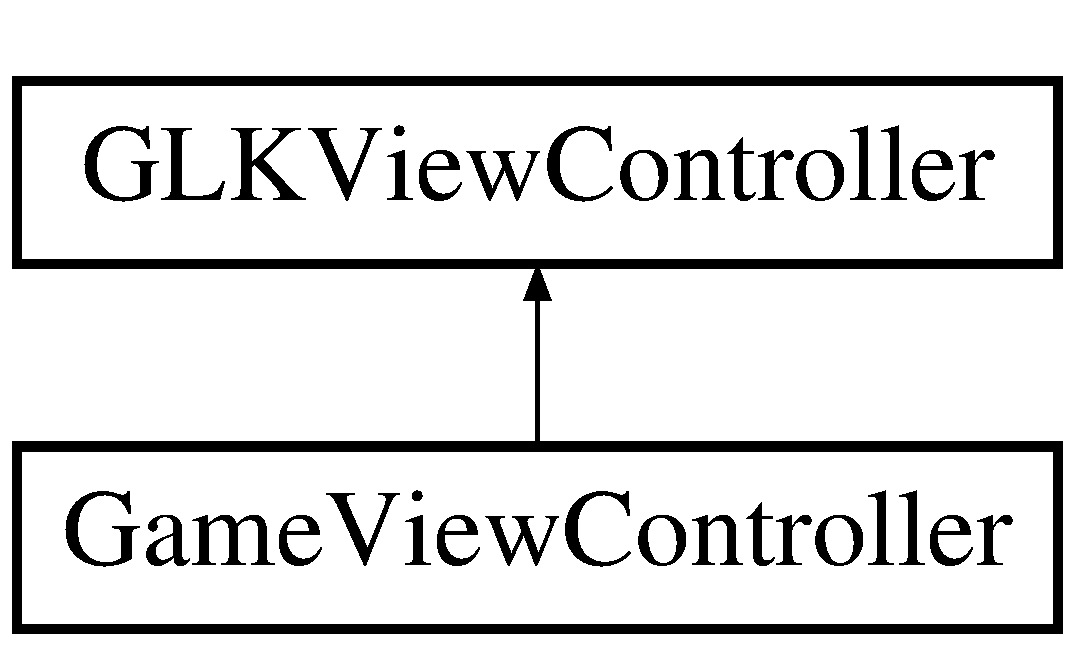
\includegraphics[height=2.000000cm]{interface_game_view_controller}
\end{center}
\end{figure}


The documentation for this class was generated from the following file\+:\begin{DoxyCompactItemize}
\item 
Game\+Engine/\+Controllers/Game\+View\+Controller.\+h\end{DoxyCompactItemize}

\hypertarget{category_game_view_controller_07_08}{}\section{Game\+View\+Controller() Category Reference}
\label{category_game_view_controller_07_08}\index{Game\+View\+Controller()@{Game\+View\+Controller()}}
\subsection*{Instance Methods}
\begin{DoxyCompactItemize}
\item 
(void) -\/ {\bfseries setup\+GL}\hypertarget{category_game_view_controller_07_08_a428d90a43c8732d980daa878bc0b796e}{}\label{category_game_view_controller_07_08_a428d90a43c8732d980daa878bc0b796e}

\item 
(void) -\/ {\bfseries tear\+Down\+GL}\hypertarget{category_game_view_controller_07_08_a126aab10acd38763920483fed64068ce}{}\label{category_game_view_controller_07_08_a126aab10acd38763920483fed64068ce}

\end{DoxyCompactItemize}
\subsection*{Protected Attributes}
\begin{DoxyCompactItemize}
\item 
G\+L\+K\+Matrix4 {\bfseries \+\_\+model\+View\+Projection\+Matrix}\hypertarget{category_game_view_controller_07_08_afc4fc1314206c1e92d45a8ec848c0b3b}{}\label{category_game_view_controller_07_08_afc4fc1314206c1e92d45a8ec848c0b3b}

\item 
G\+L\+K\+Matrix3 {\bfseries \+\_\+normal\+Matrix}\hypertarget{category_game_view_controller_07_08_a87988e8a48e8173b6ea83ffb39183e05}{}\label{category_game_view_controller_07_08_a87988e8a48e8173b6ea83ffb39183e05}

\item 
float {\bfseries \+\_\+rotation}\hypertarget{category_game_view_controller_07_08_aace8109299beb90fbd3d5239fc8bb604}{}\label{category_game_view_controller_07_08_aace8109299beb90fbd3d5239fc8bb604}

\item 
\hyperlink{interface_entity_shader_manager}{Entity\+Shader\+Manager} $\ast$ {\bfseries e\+Shader}\hypertarget{category_game_view_controller_07_08_aa65130f2cf26c4572910ccc0c5334007}{}\label{category_game_view_controller_07_08_aa65130f2cf26c4572910ccc0c5334007}

\item 
\hyperlink{interface_loader}{Loader} $\ast$ {\bfseries loader}\hypertarget{category_game_view_controller_07_08_a39ed19c46c0425a8804f79e770dd6468}{}\label{category_game_view_controller_07_08_a39ed19c46c0425a8804f79e770dd6468}

\item 
\hyperlink{interface_raw_model}{Raw\+Model} $\ast$ {\bfseries raw\+Model}\hypertarget{category_game_view_controller_07_08_aeded52f4f281027ac274883b781345c5}{}\label{category_game_view_controller_07_08_aeded52f4f281027ac274883b781345c5}

\item 
\hyperlink{interface_master_render}{Master\+Render} $\ast$ {\bfseries renderer}\hypertarget{category_game_view_controller_07_08_aaa575ada3569e8d87dc915fcf9df12a7}{}\label{category_game_view_controller_07_08_aaa575ada3569e8d87dc915fcf9df12a7}

\end{DoxyCompactItemize}
\subsection*{Properties}
\begin{DoxyCompactItemize}
\item 
E\+A\+G\+L\+Context $\ast$ {\bfseries context}\hypertarget{category_game_view_controller_07_08_a0faae9bb6914ccd71c8550177f95d41c}{}\label{category_game_view_controller_07_08_a0faae9bb6914ccd71c8550177f95d41c}

\end{DoxyCompactItemize}


The documentation for this category was generated from the following file\+:\begin{DoxyCompactItemize}
\item 
Game\+Engine/\+Controllers/Game\+View\+Controller.\+m\end{DoxyCompactItemize}

\hypertarget{interface_g_l_s_l_utils}{}\section{G\+L\+S\+L\+Utils Class Reference}
\label{interface_g_l_s_l_utils}\index{G\+L\+S\+L\+Utils@{G\+L\+S\+L\+Utils}}
Inheritance diagram for G\+L\+S\+L\+Utils\+:\begin{figure}[H]
\begin{center}
\leavevmode
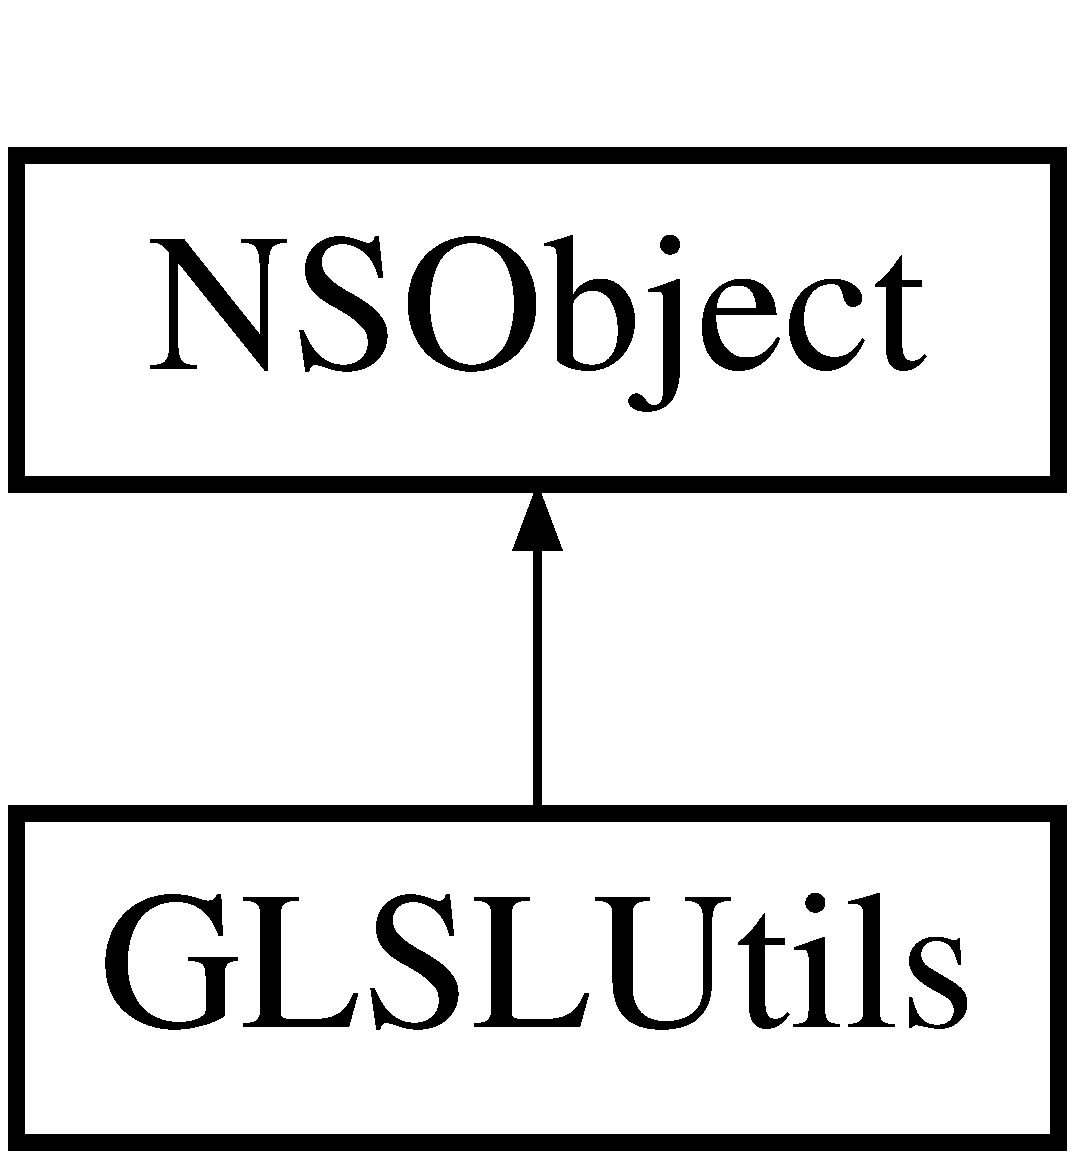
\includegraphics[height=2.000000cm]{interface_g_l_s_l_utils}
\end{center}
\end{figure}
\subsection*{Class Methods}
\begin{DoxyCompactItemize}
\item 
(\hyperlink{interface_shader_program}{Shader\+Program} $\ast$) + \hyperlink{interface_g_l_s_l_utils_afc49711c907879c1b90293a5f21e29d6}{load\+Program\+::}
\item 
(B\+O\+OL) + \hyperlink{interface_g_l_s_l_utils_a1c9c56108270842e463fe3d894e1334a}{link\+Program\+:}
\end{DoxyCompactItemize}


\subsection{Method Documentation}
\index{G\+L\+S\+L\+Utils@{G\+L\+S\+L\+Utils}!link\+Program\+:@{link\+Program\+:}}
\index{link\+Program\+:@{link\+Program\+:}!G\+L\+S\+L\+Utils@{G\+L\+S\+L\+Utils}}
\subsubsection[{\texorpdfstring{link\+Program\+:(\+Shader\+Program $\ast$shader\+Program)}{linkProgram:(ShaderProgram *shaderProgram)}}]{\setlength{\rightskip}{0pt plus 5cm}+ (B\+O\+OL) link\+Program\+: 
\begin{DoxyParamCaption}
\item[{({\bf Shader\+Program}$\ast$)}]{shader\+Program}
\end{DoxyParamCaption}
}\hypertarget{interface_g_l_s_l_utils_a1c9c56108270842e463fe3d894e1334a}{}\label{interface_g_l_s_l_utils_a1c9c56108270842e463fe3d894e1334a}
Link the program shader with their vertex shader and fragment shader


\begin{DoxyParams}{Parameters}
{\em shader\+Program} & The program shader not linked yet\\
\hline
\end{DoxyParams}
\begin{DoxyReturn}{Returns}
False = Not linked True = Linked 
\end{DoxyReturn}
\index{G\+L\+S\+L\+Utils@{G\+L\+S\+L\+Utils}!load\+Program\+::@{load\+Program\+::}}
\index{load\+Program\+::@{load\+Program\+::}!G\+L\+S\+L\+Utils@{G\+L\+S\+L\+Utils}}
\subsubsection[{\texorpdfstring{load\+Program\+::(const char $\ast$vertex\+Shader\+Src,[] const char $\ast$frag\+Shader\+Src)}{loadProgram::(const char *vertexShaderSrc,[] const char *fragShaderSrc)}}]{\setlength{\rightskip}{0pt plus 5cm}+ ({\bf Shader\+Program} $\ast$) load\+Program\+: 
\begin{DoxyParamCaption}
\item[{(const char $\ast$)}]{vertex\+Shader\+Src}
\item[{:(const char $\ast$)}]{frag\+Shader\+Src}
\end{DoxyParamCaption}
}\hypertarget{interface_g_l_s_l_utils_afc49711c907879c1b90293a5f21e29d6}{}\label{interface_g_l_s_l_utils_afc49711c907879c1b90293a5f21e29d6}
Compiles the shader sources and attache them to the program


\begin{DoxyParams}{Parameters}
{\em vertex\+Shader\+Src} & Source code of the vertex shader \\
\hline
{\em frag\+Shader\+Src} & Source code of the fragment shader \\
\hline
\end{DoxyParams}
\begin{DoxyReturn}{Returns}
nil There was an error not 0 -\/$>$ Id of the program loaded 
\end{DoxyReturn}


The documentation for this class was generated from the following files\+:\begin{DoxyCompactItemize}
\item 
Game\+Engine/\+Commons/G\+L\+S\+L\+Utils.\+h\item 
Game\+Engine/\+Commons/G\+L\+S\+L\+Utils.\+m\end{DoxyCompactItemize}

\hypertarget{protocol_i_shape-p}{}\section{$<$I\+Shape$>$ Protocol Reference}
\label{protocol_i_shape-p}\index{$<$\+I\+Shape$>$@{$<$\+I\+Shape$>$}}


{\ttfamily \#import $<$I\+Shape.\+h$>$}

Inheritance diagram for $<$I\+Shape$>$\+:\begin{figure}[H]
\begin{center}
\leavevmode
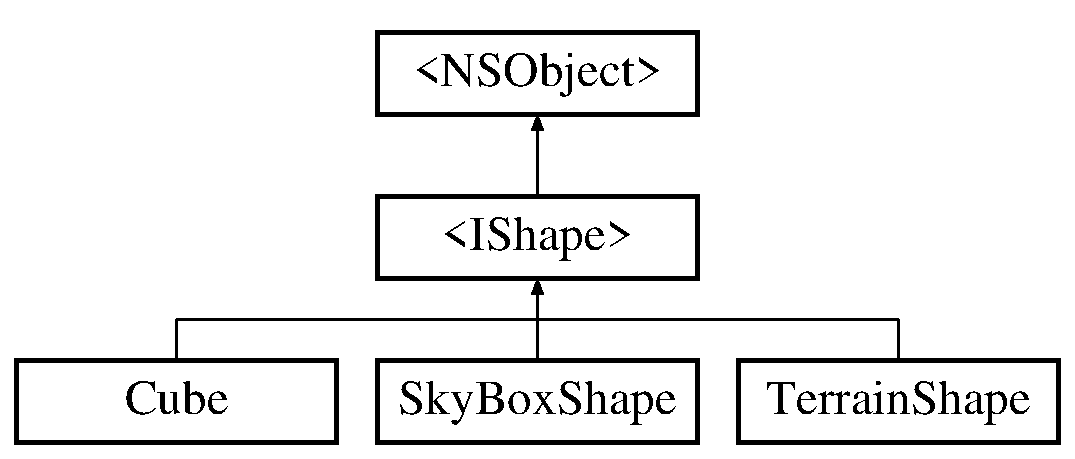
\includegraphics[height=3.000000cm]{protocol_i_shape-p}
\end{center}
\end{figure}
\subsection*{Instance Methods}
\begin{DoxyCompactItemize}
\item 
(float($\ast$) -\/ \hyperlink{protocol_i_shape-p_a0d22f432f5a46500a7264f71cc6c1aa0}{get\+Vertices}
\item 
(int) -\/ \hyperlink{protocol_i_shape-p_ac0953f79b242f614b8d0d4bbee7c78ec}{count\+Vertices}
\item 
(float $\ast$) -\/ \hyperlink{protocol_i_shape-p_a0dfdefe0e8402efcdaac08542b4e2657}{get\+Texture\+Coords}
\item 
(int) -\/ {\bfseries count\+Texture\+Coords}\hypertarget{protocol_i_shape-p_a67a5bb73ff327adf2867882e0a14415a}{}\label{protocol_i_shape-p_a67a5bb73ff327adf2867882e0a14415a}

\item 
(float $\ast$) -\/ \hyperlink{protocol_i_shape-p_a26b9453056e6fdceae7f413ce5648035}{get\+Normals}
\item 
(int) -\/ {\bfseries count\+Normals}\hypertarget{protocol_i_shape-p_ae4466484cab2e1d256ec4de865459376}{}\label{protocol_i_shape-p_ae4466484cab2e1d256ec4de865459376}

\item 
(int $\ast$) -\/ \hyperlink{protocol_i_shape-p_a514418ae840ad3711ea8f99962ec9974}{get\+Indices}
\item 
(int) -\/ {\bfseries count\+Indices}\hypertarget{protocol_i_shape-p_a3154097fa193edfd42625f3286c24321}{}\label{protocol_i_shape-p_a3154097fa193edfd42625f3286c24321}

\end{DoxyCompactItemize}


\subsection{Detailed Description}
Interface that should be implemented for the different shapes available 

\subsection{Method Documentation}
\index{I\+Shape-\/p@{I\+Shape-\/p}!count\+Vertices@{count\+Vertices}}
\index{count\+Vertices@{count\+Vertices}!I\+Shape-\/p@{I\+Shape-\/p}}
\subsubsection[{\texorpdfstring{count\+Vertices()}{countVertices()}}]{\setlength{\rightskip}{0pt plus 5cm}-\/ (int) count\+Vertices 
\begin{DoxyParamCaption}
{}
\end{DoxyParamCaption}
}\hypertarget{protocol_i_shape-p_ac0953f79b242f614b8d0d4bbee7c78ec}{}\label{protocol_i_shape-p_ac0953f79b242f614b8d0d4bbee7c78ec}
\begin{DoxyReturn}{Returns}
number of vertices that make the shape 
\end{DoxyReturn}
\index{I\+Shape-\/p@{I\+Shape-\/p}!get\+Indices@{get\+Indices}}
\index{get\+Indices@{get\+Indices}!I\+Shape-\/p@{I\+Shape-\/p}}
\subsubsection[{\texorpdfstring{get\+Indices()}{getIndices()}}]{\setlength{\rightskip}{0pt plus 5cm}-\/ (int$\ast$) get\+Indices 
\begin{DoxyParamCaption}
{}
\end{DoxyParamCaption}
}\hypertarget{protocol_i_shape-p_a514418ae840ad3711ea8f99962ec9974}{}\label{protocol_i_shape-p_a514418ae840ad3711ea8f99962ec9974}
\begin{DoxyReturn}{Returns}
The indices of the vertices that make the shape 
\end{DoxyReturn}
\index{I\+Shape-\/p@{I\+Shape-\/p}!get\+Normals@{get\+Normals}}
\index{get\+Normals@{get\+Normals}!I\+Shape-\/p@{I\+Shape-\/p}}
\subsubsection[{\texorpdfstring{get\+Normals()}{getNormals()}}]{\setlength{\rightskip}{0pt plus 5cm}-\/ (float$\ast$) get\+Normals 
\begin{DoxyParamCaption}
{}
\end{DoxyParamCaption}
}\hypertarget{protocol_i_shape-p_a26b9453056e6fdceae7f413ce5648035}{}\label{protocol_i_shape-p_a26b9453056e6fdceae7f413ce5648035}
\begin{DoxyReturn}{Returns}
the normal vectors that make the shape 
\end{DoxyReturn}
\index{I\+Shape-\/p@{I\+Shape-\/p}!get\+Texture\+Coords@{get\+Texture\+Coords}}
\index{get\+Texture\+Coords@{get\+Texture\+Coords}!I\+Shape-\/p@{I\+Shape-\/p}}
\subsubsection[{\texorpdfstring{get\+Texture\+Coords()}{getTextureCoords()}}]{\setlength{\rightskip}{0pt plus 5cm}-\/ (float$\ast$) get\+Texture\+Coords 
\begin{DoxyParamCaption}
{}
\end{DoxyParamCaption}
}\hypertarget{protocol_i_shape-p_a0dfdefe0e8402efcdaac08542b4e2657}{}\label{protocol_i_shape-p_a0dfdefe0e8402efcdaac08542b4e2657}
\begin{DoxyReturn}{Returns}
the Coordinates of the textures of the shape 
\end{DoxyReturn}
\index{I\+Shape-\/p@{I\+Shape-\/p}!get\+Vertices@{get\+Vertices}}
\index{get\+Vertices@{get\+Vertices}!I\+Shape-\/p@{I\+Shape-\/p}}
\subsubsection[{\texorpdfstring{get\+Vertices()}{getVertices()}}]{\setlength{\rightskip}{0pt plus 5cm}-\/ (float($\ast$) get\+Vertices 
\begin{DoxyParamCaption}
{}
\end{DoxyParamCaption}
}\hypertarget{protocol_i_shape-p_a0d22f432f5a46500a7264f71cc6c1aa0}{}\label{protocol_i_shape-p_a0d22f432f5a46500a7264f71cc6c1aa0}
\begin{DoxyReturn}{Returns}
the vertices of the shape 
\end{DoxyReturn}


The documentation for this protocol was generated from the following file\+:\begin{DoxyCompactItemize}
\item 
Game\+Engine/\+Shapes/I\+Shape.\+h\end{DoxyCompactItemize}

\hypertarget{interface_loader}{}\section{Loader Class Reference}
\label{interface_loader}\index{Loader@{Loader}}
Inheritance diagram for Loader\+:\begin{figure}[H]
\begin{center}
\leavevmode
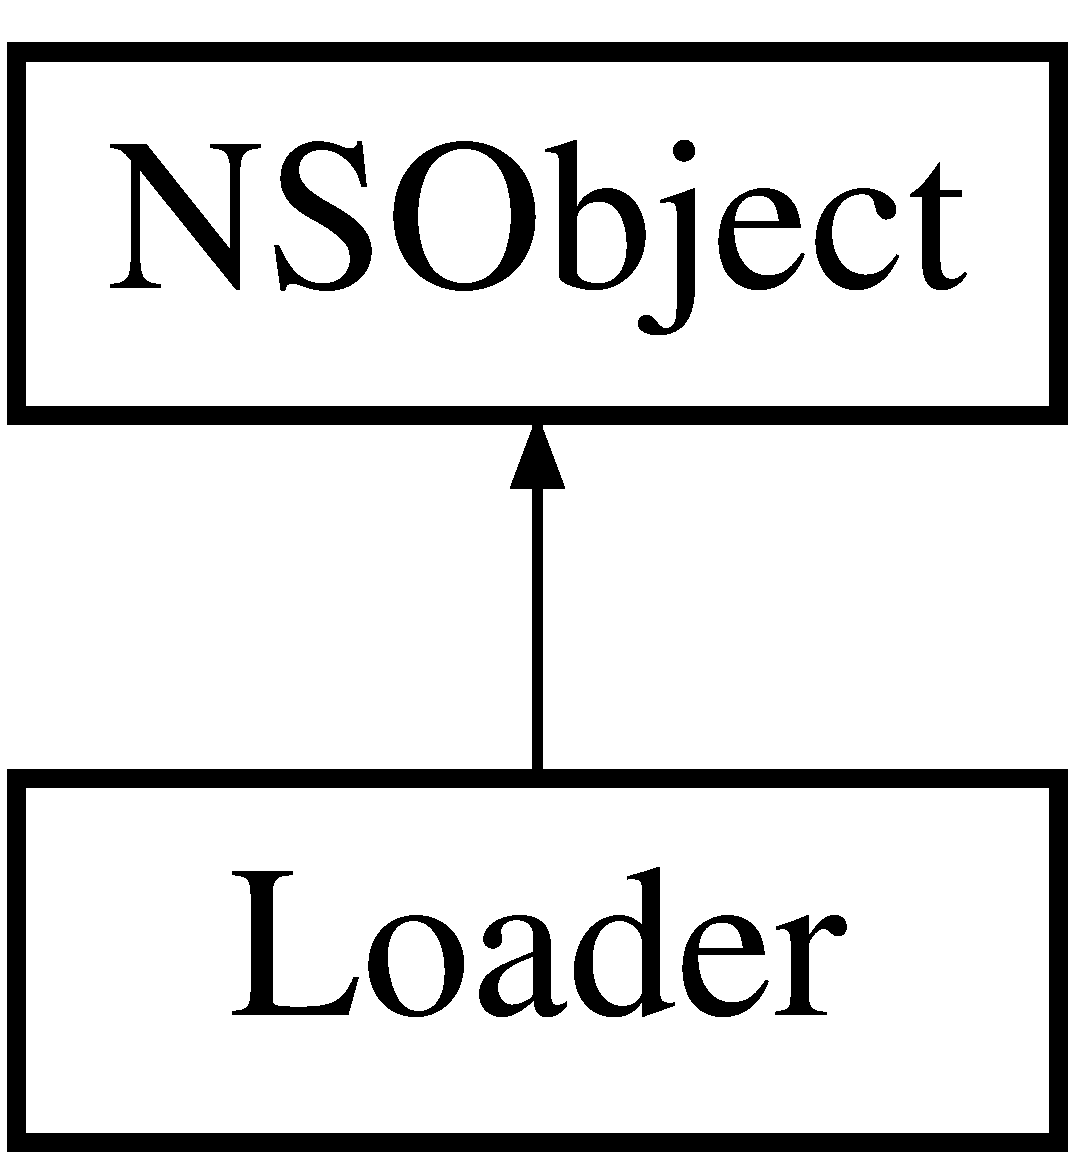
\includegraphics[height=2.000000cm]{interface_loader}
\end{center}
\end{figure}
\subsection*{Instance Methods}
\begin{DoxyCompactItemize}
\item 
(id) -\/ \hyperlink{interface_loader_a0de390987e7d3e88f5e22c4ba81fbbb1}{init}
\item 
(\hyperlink{interface_raw_model}{Raw\+Model} $\ast$) -\/ \hyperlink{interface_loader_a1d77fb9c5b8461d4f6c7d26a0c0c598b}{load\+To\+V\+A\+O\+:}
\end{DoxyCompactItemize}


\subsection{Method Documentation}
\index{Loader@{Loader}!init@{init}}
\index{init@{init}!Loader@{Loader}}
\subsubsection[{\texorpdfstring{init()}{init()}}]{\setlength{\rightskip}{0pt plus 5cm}-\/ (id) init 
\begin{DoxyParamCaption}
{}
\end{DoxyParamCaption}
}\hypertarget{interface_loader_a0de390987e7d3e88f5e22c4ba81fbbb1}{}\label{interface_loader_a0de390987e7d3e88f5e22c4ba81fbbb1}
Initiator of the loader \index{Loader@{Loader}!load\+To\+V\+A\+O\+:@{load\+To\+V\+A\+O\+:}}
\index{load\+To\+V\+A\+O\+:@{load\+To\+V\+A\+O\+:}!Loader@{Loader}}
\subsubsection[{\texorpdfstring{load\+To\+V\+A\+O\+:(id$<$ I\+Shape $>$ shape)}{loadToVAO:(id< IShape > shape)}}]{\setlength{\rightskip}{0pt plus 5cm}-\/ ({\bf Raw\+Model} $\ast$) load\+To\+V\+A\+O\+: 
\begin{DoxyParamCaption}
\item[{(id$<${\bf I\+Shape}$>$)}]{shape}
\end{DoxyParamCaption}
}\hypertarget{interface_loader_a1d77fb9c5b8461d4f6c7d26a0c0c598b}{}\label{interface_loader_a1d77fb9c5b8461d4f6c7d26a0c0c598b}
Load to a new vertex array object


\begin{DoxyParams}{Parameters}
{\em shape} & The shape to load\\
\hline
\end{DoxyParams}
\begin{DoxyReturn}{Returns}
A row model with information loaded 
\end{DoxyReturn}


The documentation for this class was generated from the following files\+:\begin{DoxyCompactItemize}
\item 
Game\+Engine/\+Render\+Engine/Loader.\+h\item 
Game\+Engine/\+Render\+Engine/Loader.\+m\end{DoxyCompactItemize}

\hypertarget{interface_load_utils}{}\section{Load\+Utils Class Reference}
\label{interface_load_utils}\index{Load\+Utils@{Load\+Utils}}
Inheritance diagram for Load\+Utils\+:\begin{figure}[H]
\begin{center}
\leavevmode
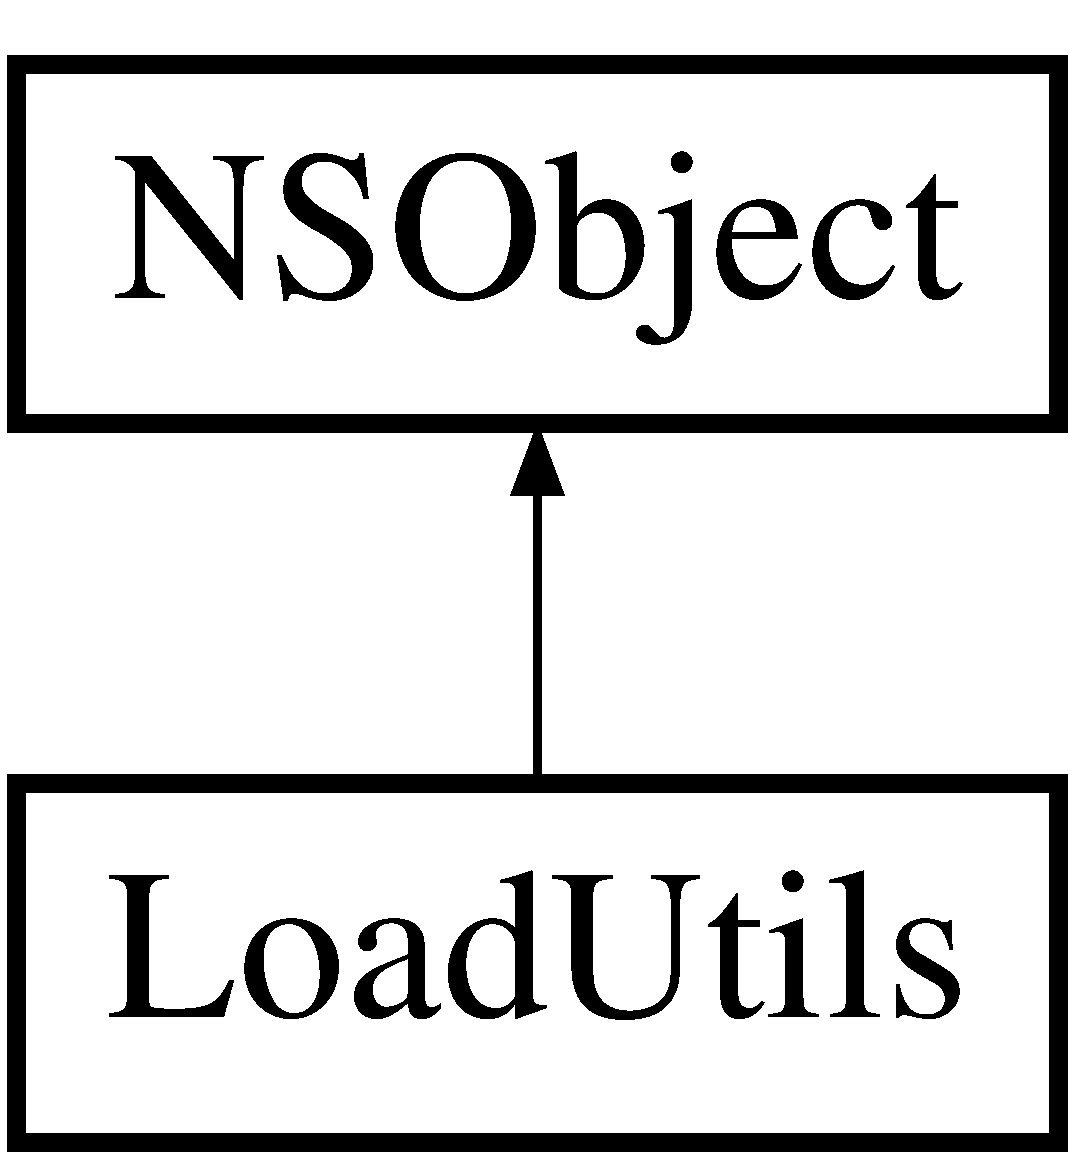
\includegraphics[height=2.000000cm]{interface_load_utils}
\end{center}
\end{figure}
\subsection*{Class Methods}
\begin{DoxyCompactItemize}
\item 
(const char $\ast$) + \hyperlink{interface_load_utils_aa29e9e6d99aa21a9d60cf465e124f2bc}{read\+Text\+From\+Raw\+Resource\+:}
\end{DoxyCompactItemize}


\subsection{Method Documentation}
\index{Load\+Utils@{Load\+Utils}!read\+Text\+From\+Raw\+Resource\+:@{read\+Text\+From\+Raw\+Resource\+:}}
\index{read\+Text\+From\+Raw\+Resource\+:@{read\+Text\+From\+Raw\+Resource\+:}!Load\+Utils@{Load\+Utils}}
\subsubsection[{\texorpdfstring{read\+Text\+From\+Raw\+Resource\+:(\+N\+S\+String $\ast$file\+Name)}{readTextFromRawResource:(NSString *fileName)}}]{\setlength{\rightskip}{0pt plus 5cm}+ (const char $\ast$) read\+Text\+From\+Raw\+Resource\+: 
\begin{DoxyParamCaption}
\item[{(N\+S\+String$\ast$)}]{file\+Name}
\end{DoxyParamCaption}
}\hypertarget{interface_load_utils_aa29e9e6d99aa21a9d60cf465e124f2bc}{}\label{interface_load_utils_aa29e9e6d99aa21a9d60cf465e124f2bc}
Reads a string from a certain resource


\begin{DoxyParams}{Parameters}
{\em file\+Name} & id of the resource where the text exists \\
\hline
\end{DoxyParams}
\begin{DoxyReturn}{Returns}
The text that exists in the resource 
\end{DoxyReturn}


The documentation for this class was generated from the following files\+:\begin{DoxyCompactItemize}
\item 
Game\+Engine/\+Commons/Load\+Utils.\+h\item 
Game\+Engine/\+Commons/Load\+Utils.\+m\end{DoxyCompactItemize}

\hypertarget{interface_master_render}{}\section{Master\+Render Class Reference}
\label{interface_master_render}\index{Master\+Render@{Master\+Render}}


{\ttfamily \#import $<$Master\+Render.\+h$>$}

Inheritance diagram for Master\+Render\+:\begin{figure}[H]
\begin{center}
\leavevmode
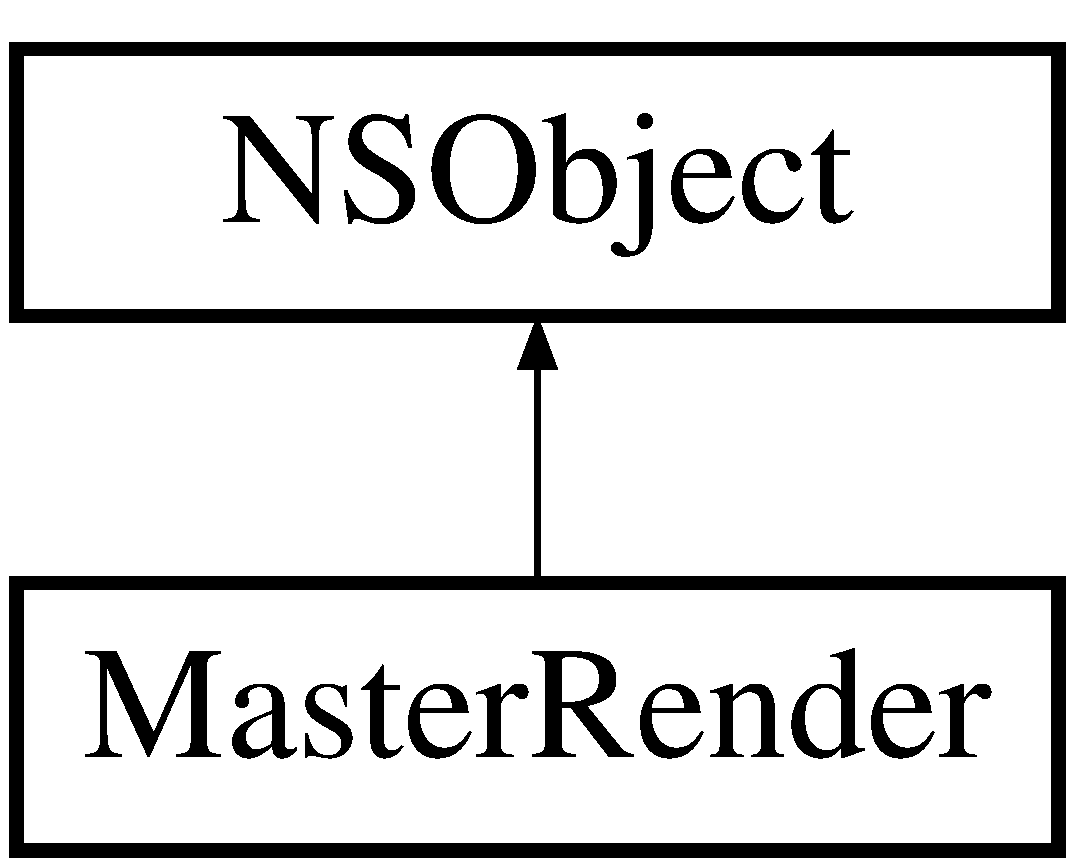
\includegraphics[height=2.000000cm]{interface_master_render}
\end{center}
\end{figure}
\subsection*{Instance Methods}
\begin{DoxyCompactItemize}
\item 
(id) -\/ \hyperlink{interface_master_render_a695e7537040ffa21d5c12cb53959fe94}{init\+::}
\item 
(G\+L\+K\+Matrix4) -\/ \hyperlink{interface_master_render_a9b982f26c9c6f590fc13ba565138301c}{create\+Projection\+Matrix}
\item 
(G\+L\+K\+Matrix4) -\/ \hyperlink{interface_master_render_ae641cf62f29a9785af6e4c827e7951e0}{update\+Camera}
\item 
(void) -\/ \hyperlink{interface_master_render_aabbf9dc1b344e9050f3ad35f383414de}{render}
\end{DoxyCompactItemize}


\subsection{Detailed Description}
Groups the entities in a hash map like this the same entity will be just put in different positions 

\subsection{Method Documentation}
\index{Master\+Render@{Master\+Render}!create\+Projection\+Matrix@{create\+Projection\+Matrix}}
\index{create\+Projection\+Matrix@{create\+Projection\+Matrix}!Master\+Render@{Master\+Render}}
\subsubsection[{\texorpdfstring{create\+Projection\+Matrix()}{createProjectionMatrix()}}]{\setlength{\rightskip}{0pt plus 5cm}-\/ (G\+L\+K\+Matrix4) create\+Projection\+Matrix 
\begin{DoxyParamCaption}
{}
\end{DoxyParamCaption}
}\hypertarget{interface_master_render_a9b982f26c9c6f590fc13ba565138301c}{}\label{interface_master_render_a9b982f26c9c6f590fc13ba565138301c}
Create the projection matrix with parameters of the camera

\begin{DoxyReturn}{Returns}
A projection matrix 
\end{DoxyReturn}
\index{Master\+Render@{Master\+Render}!init\+::@{init\+::}}
\index{init\+::@{init\+::}!Master\+Render@{Master\+Render}}
\subsubsection[{\texorpdfstring{init\+::(int width,[] int height)}{init::(int width,[] int height)}}]{\setlength{\rightskip}{0pt plus 5cm}-\/ (id) init\+: 
\begin{DoxyParamCaption}
\item[{(int)}]{a\+Width}
\item[{:(int)}]{a\+Height}
\end{DoxyParamCaption}
}\hypertarget{interface_master_render_a695e7537040ffa21d5c12cb53959fe94}{}\label{interface_master_render_a695e7537040ffa21d5c12cb53959fe94}
Initiator of the master render \index{Master\+Render@{Master\+Render}!render@{render}}
\index{render@{render}!Master\+Render@{Master\+Render}}
\subsubsection[{\texorpdfstring{render()}{render()}}]{\setlength{\rightskip}{0pt plus 5cm}-\/ (void) render 
\begin{DoxyParamCaption}
{}
\end{DoxyParamCaption}
}\hypertarget{interface_master_render_aabbf9dc1b344e9050f3ad35f383414de}{}\label{interface_master_render_aabbf9dc1b344e9050f3ad35f383414de}
Render the entire scene (Called by each frame)


\begin{DoxyParams}{Parameters}
{\em sun} & Sun of the scene \\
\hline
\end{DoxyParams}
\index{Master\+Render@{Master\+Render}!update\+Camera@{update\+Camera}}
\index{update\+Camera@{update\+Camera}!Master\+Render@{Master\+Render}}
\subsubsection[{\texorpdfstring{update\+Camera()}{updateCamera()}}]{\setlength{\rightskip}{0pt plus 5cm}-\/ (G\+L\+K\+Matrix4) update\+Camera 
\begin{DoxyParamCaption}
{}
\end{DoxyParamCaption}
}\hypertarget{interface_master_render_ae641cf62f29a9785af6e4c827e7951e0}{}\label{interface_master_render_ae641cf62f29a9785af6e4c827e7951e0}
Calls the methods to update the camera and updates the matrix that describe the camera in the scene 

The documentation for this class was generated from the following files\+:\begin{DoxyCompactItemize}
\item 
Game\+Engine/\+Render\+Engine/Master\+Render.\+h\item 
Game\+Engine/\+Render\+Engine/Master\+Render.\+m\end{DoxyCompactItemize}

\hypertarget{interface_model_texture}{}\section{Model\+Texture Class Reference}
\label{interface_model_texture}\index{Model\+Texture@{Model\+Texture}}


{\ttfamily \#import $<$Model\+Texture.\+h$>$}

Inheritance diagram for Model\+Texture\+:\begin{figure}[H]
\begin{center}
\leavevmode
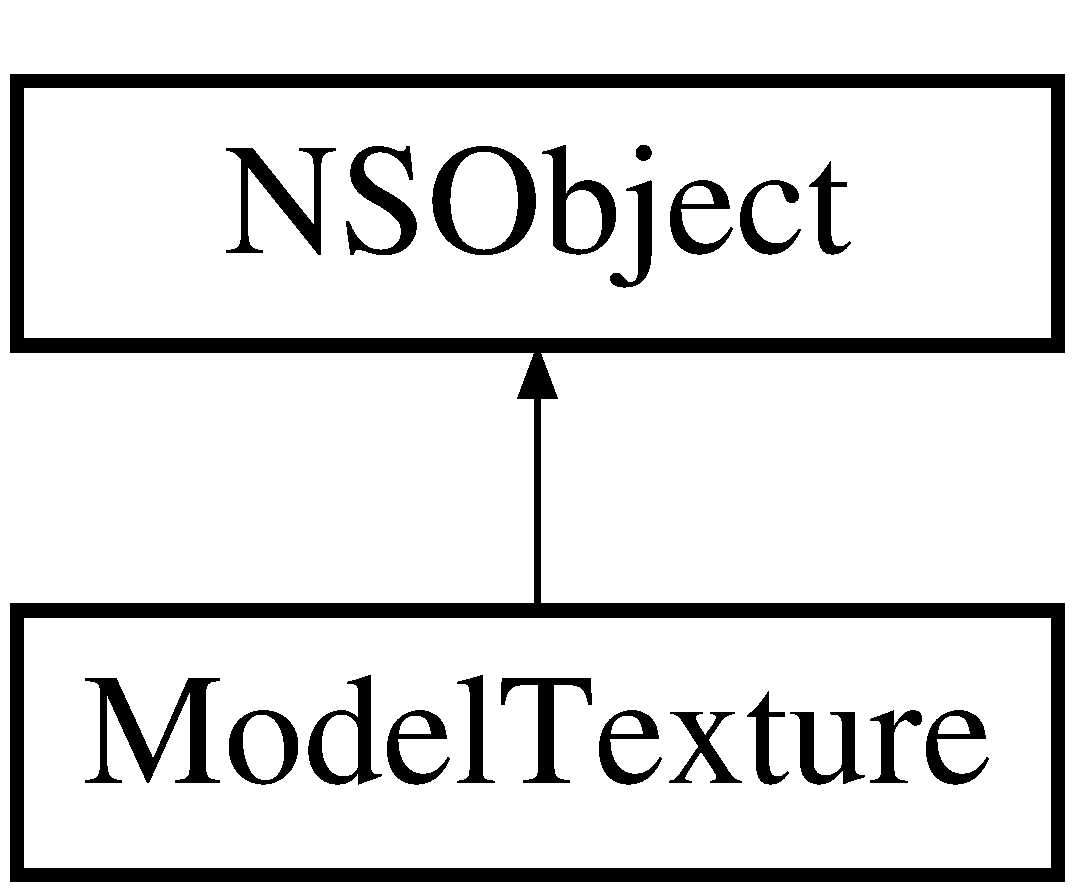
\includegraphics[height=2.000000cm]{interface_model_texture}
\end{center}
\end{figure}
\subsection*{Properties}
\begin{DoxyCompactItemize}
\item 
int \hyperlink{interface_model_texture_a6036cd5d7473640c480a385695dba581}{texture\+Id}
\item 
float \hyperlink{interface_model_texture_ad9d65575408a2195c3c8a654e804e8ce}{shine\+Damper}
\item 
float \hyperlink{interface_model_texture_a61a956a6fad9b4686c7299ea8f3f76c7}{reflectivity}
\end{DoxyCompactItemize}


\subsection{Detailed Description}
Has all the required parameters to render one textured entity 

\subsection{Property Documentation}
\index{Model\+Texture@{Model\+Texture}!reflectivity@{reflectivity}}
\index{reflectivity@{reflectivity}!Model\+Texture@{Model\+Texture}}
\subsubsection[{\texorpdfstring{reflectivity}{reflectivity}}]{\setlength{\rightskip}{0pt plus 5cm}-\/ (float) reflectivity\hspace{0.3cm}{\ttfamily [read]}, {\ttfamily [write]}, {\ttfamily [atomic]}}\hypertarget{interface_model_texture_a61a956a6fad9b4686c7299ea8f3f76c7}{}\label{interface_model_texture_a61a956a6fad9b4686c7299ea8f3f76c7}
How reflective the model is \index{Model\+Texture@{Model\+Texture}!shine\+Damper@{shine\+Damper}}
\index{shine\+Damper@{shine\+Damper}!Model\+Texture@{Model\+Texture}}
\subsubsection[{\texorpdfstring{shine\+Damper}{shineDamper}}]{\setlength{\rightskip}{0pt plus 5cm}-\/ (float) shine\+Damper\hspace{0.3cm}{\ttfamily [read]}, {\ttfamily [write]}, {\ttfamily [atomic]}}\hypertarget{interface_model_texture_ad9d65575408a2195c3c8a654e804e8ce}{}\label{interface_model_texture_ad9d65575408a2195c3c8a654e804e8ce}
How damped the shine is \index{Model\+Texture@{Model\+Texture}!texture\+Id@{texture\+Id}}
\index{texture\+Id@{texture\+Id}!Model\+Texture@{Model\+Texture}}
\subsubsection[{\texorpdfstring{texture\+Id}{textureId}}]{\setlength{\rightskip}{0pt plus 5cm}-\/ (int) texture\+Id\hspace{0.3cm}{\ttfamily [read]}, {\ttfamily [write]}, {\ttfamily [atomic]}}\hypertarget{interface_model_texture_a6036cd5d7473640c480a385695dba581}{}\label{interface_model_texture_a6036cd5d7473640c480a385695dba581}
The identifier of the texture 

The documentation for this class was generated from the following file\+:\begin{DoxyCompactItemize}
\item 
Game\+Engine/\+Textures/Model\+Texture.\+h\end{DoxyCompactItemize}

\hypertarget{interface_raw_model}{}\section{Raw\+Model Class Reference}
\label{interface_raw_model}\index{Raw\+Model@{Raw\+Model}}
Inheritance diagram for Raw\+Model\+:\begin{figure}[H]
\begin{center}
\leavevmode
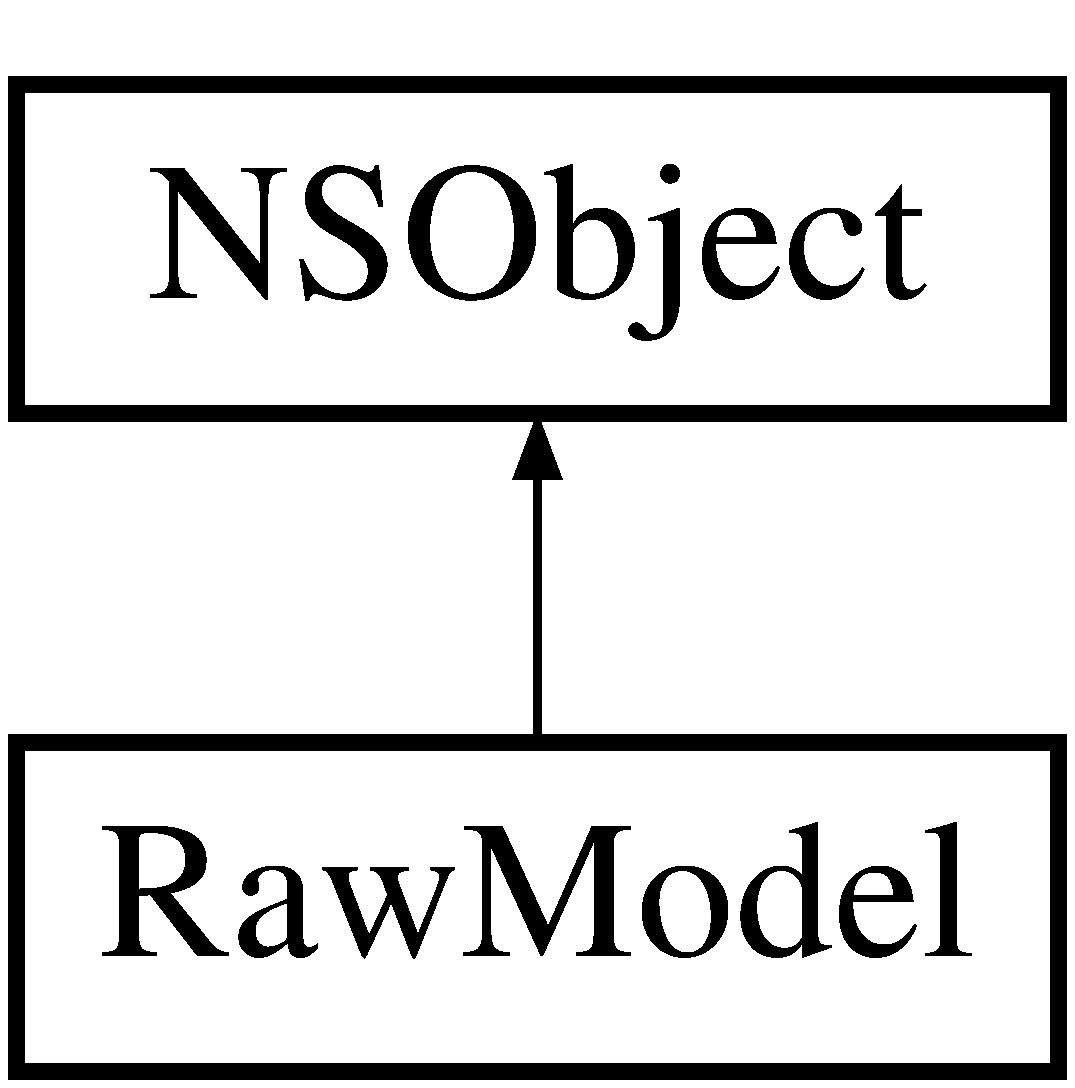
\includegraphics[height=2.000000cm]{interface_raw_model}
\end{center}
\end{figure}
\subsection*{Instance Methods}
\begin{DoxyCompactItemize}
\item 
(id) -\/ \hyperlink{interface_raw_model_a4d75722dec3db7a09a5bde18b3a3118e}{init\+::}
\end{DoxyCompactItemize}
\subsection*{Properties}
\begin{DoxyCompactItemize}
\item 
int \hyperlink{interface_raw_model_a136659c909db791eabf42a7f63449337}{vao\+Id}
\item 
int \hyperlink{interface_raw_model_adc187504bcabe21832acfb0df3103711}{vertex\+Count}
\end{DoxyCompactItemize}


\subsection{Method Documentation}
\index{Raw\+Model@{Raw\+Model}!init\+::@{init\+::}}
\index{init\+::@{init\+::}!Raw\+Model@{Raw\+Model}}
\subsubsection[{\texorpdfstring{init\+::(int a\+Vao\+Id,[] int a\+Vertex\+Count)}{init::(int aVaoId,[] int aVertexCount)}}]{\setlength{\rightskip}{0pt plus 5cm}-\/ (id) init\+: 
\begin{DoxyParamCaption}
\item[{(int)}]{a\+Vao\+Id}
\item[{:(int)}]{a\+Vertex\+Count}
\end{DoxyParamCaption}
}\hypertarget{interface_raw_model_a4d75722dec3db7a09a5bde18b3a3118e}{}\label{interface_raw_model_a4d75722dec3db7a09a5bde18b3a3118e}
Initiator of the raw model


\begin{DoxyParams}{Parameters}
{\em the} & vao\+Id assigned by open\+GL \\
\hline
{\em the} & number of vertex \\
\hline
\end{DoxyParams}


\subsection{Property Documentation}
\index{Raw\+Model@{Raw\+Model}!vao\+Id@{vao\+Id}}
\index{vao\+Id@{vao\+Id}!Raw\+Model@{Raw\+Model}}
\subsubsection[{\texorpdfstring{vao\+Id}{vaoId}}]{\setlength{\rightskip}{0pt plus 5cm}-\/ (int) vao\+Id\hspace{0.3cm}{\ttfamily [read]}, {\ttfamily [atomic]}, {\ttfamily [assign]}}\hypertarget{interface_raw_model_a136659c909db791eabf42a7f63449337}{}\label{interface_raw_model_a136659c909db791eabf42a7f63449337}
Identifier of the vertex array object of the raw model \index{Raw\+Model@{Raw\+Model}!vertex\+Count@{vertex\+Count}}
\index{vertex\+Count@{vertex\+Count}!Raw\+Model@{Raw\+Model}}
\subsubsection[{\texorpdfstring{vertex\+Count}{vertexCount}}]{\setlength{\rightskip}{0pt plus 5cm}-\/ (int) vertex\+Count\hspace{0.3cm}{\ttfamily [read]}, {\ttfamily [atomic]}, {\ttfamily [assign]}}\hypertarget{interface_raw_model_adc187504bcabe21832acfb0df3103711}{}\label{interface_raw_model_adc187504bcabe21832acfb0df3103711}
Number of vertices of the raw model 

The documentation for this class was generated from the following files\+:\begin{DoxyCompactItemize}
\item 
Game\+Engine/\+Models/Raw\+Model.\+h\item 
Game\+Engine/\+Models/Raw\+Model.\+m\end{DoxyCompactItemize}

\hypertarget{interface_shader_manager}{}\section{Shader\+Manager Class Reference}
\label{interface_shader_manager}\index{Shader\+Manager@{Shader\+Manager}}
Inheritance diagram for Shader\+Manager\+:\begin{figure}[H]
\begin{center}
\leavevmode
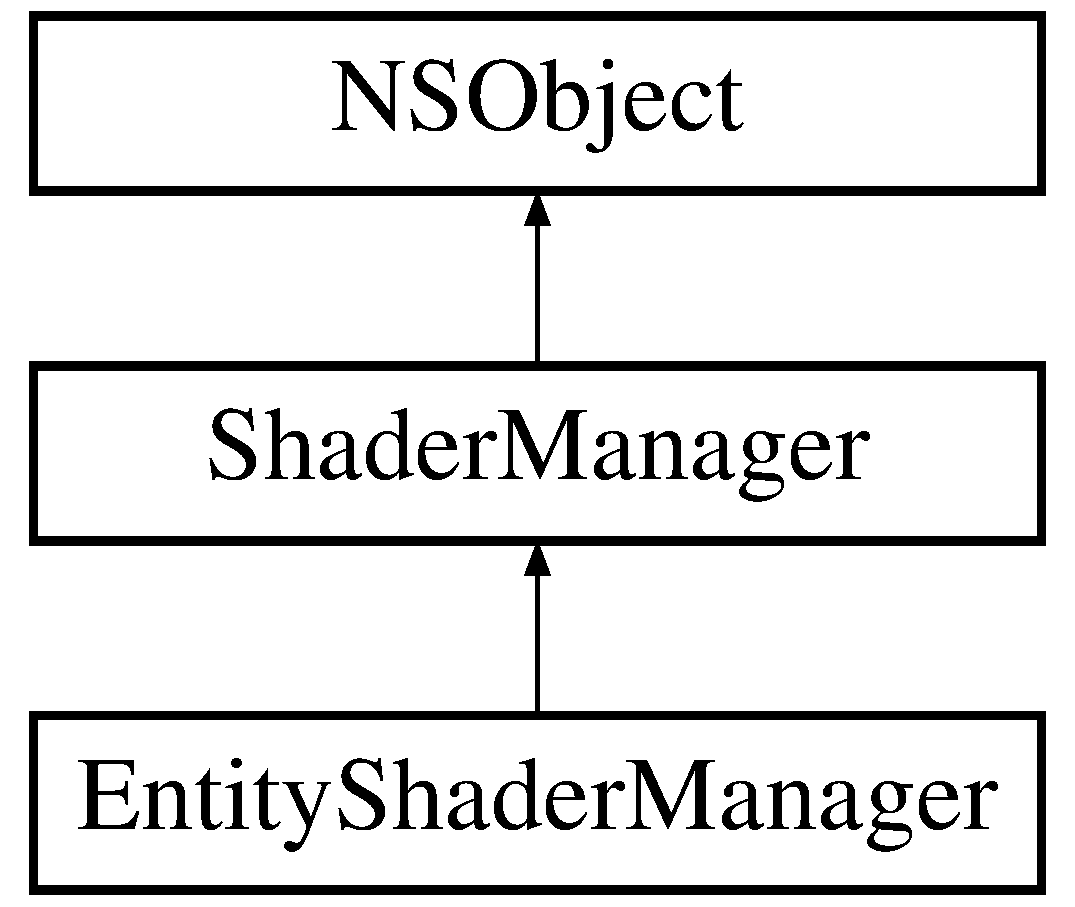
\includegraphics[height=3.000000cm]{interface_shader_manager}
\end{center}
\end{figure}
\subsection*{Instance Methods}
\begin{DoxyCompactItemize}
\item 
(id) -\/ \hyperlink{interface_shader_manager_a5b7d6903d3e8dcf4875cb144046e3262}{init\+::}
\item 
(void) -\/ \hyperlink{interface_shader_manager_ad7c264b0d06bccf7c1e19976633173d0}{bind\+Attributes}
\item 
(void) -\/ \hyperlink{interface_shader_manager_abe1fcce536c9bd78cd14a23e2b2ac46b}{get\+All\+Uniform\+Locations}
\item 
(void) -\/ \hyperlink{interface_shader_manager_a9fb731a8cd811cf1740c13cb52774f18}{bind\+Attribute\+::}
\item 
(int) -\/ \hyperlink{interface_shader_manager_a0923a8bdd737a702639f26549c2d5186}{get\+Uniform\+Location\+:}
\item 
(void) -\/ \hyperlink{interface_shader_manager_aad63531f25750d7cb657dcb10670a5c5}{load\+Int\+::}
\item 
(void) -\/ \hyperlink{interface_shader_manager_a613176179acff066ba03a1409b93dcf3}{load\+Float\+::}
\item 
(void) -\/ \hyperlink{interface_shader_manager_accbae5024b71677f3e9fef5c8b6cd0fa}{load\+Boolean\+::}
\item 
(void) -\/ \hyperlink{interface_shader_manager_a23706b17b23084ce2e83055857631905}{load\+Matrix\+::}
\item 
(void) -\/ \hyperlink{interface_shader_manager_a7dc69f2cb034c904c1483e7764cdb71b}{load\+Matrix3\+::}
\item 
(void) -\/ \hyperlink{interface_shader_manager_a5169f1f4fac9bf471bb328275d5eb6e5}{start}
\item 
(void) -\/ \hyperlink{interface_shader_manager_ade2ef03222793482549cc5f49f5f0fd3}{stop}
\item 
(void) -\/ \hyperlink{interface_shader_manager_ad0519a6e937387a7a3377123d2eac386}{dealloc}
\end{DoxyCompactItemize}


\subsection{Method Documentation}
\index{Shader\+Manager@{Shader\+Manager}!bind\+Attribute\+::@{bind\+Attribute\+::}}
\index{bind\+Attribute\+::@{bind\+Attribute\+::}!Shader\+Manager@{Shader\+Manager}}
\subsubsection[{\texorpdfstring{bind\+Attribute\+::(int attribute\+Index,[] char $\ast$variable\+Name)}{bindAttribute::(int attributeIndex,[] char *variableName)}}]{\setlength{\rightskip}{0pt plus 5cm}-\/ (void) bind\+Attribute\+: 
\begin{DoxyParamCaption}
\item[{(int)}]{attribute\+Index}
\item[{:(char$\ast$)}]{variable\+Name}
\end{DoxyParamCaption}
}\hypertarget{interface_shader_manager_a9fb731a8cd811cf1740c13cb52774f18}{}\label{interface_shader_manager_a9fb731a8cd811cf1740c13cb52774f18}
Bind one attribute


\begin{DoxyParams}{Parameters}
{\em attribute\+Index} & Index of the attribute to bind \\
\hline
{\em variable\+Name} & Name of the attribute to bind \\
\hline
\end{DoxyParams}
\index{Shader\+Manager@{Shader\+Manager}!bind\+Attributes@{bind\+Attributes}}
\index{bind\+Attributes@{bind\+Attributes}!Shader\+Manager@{Shader\+Manager}}
\subsubsection[{\texorpdfstring{bind\+Attributes()}{bindAttributes()}}]{\setlength{\rightskip}{0pt plus 5cm}-\/ (void) bind\+Attributes 
\begin{DoxyParamCaption}
{}
\end{DoxyParamCaption}
}\hypertarget{interface_shader_manager_ad7c264b0d06bccf7c1e19976633173d0}{}\label{interface_shader_manager_ad7c264b0d06bccf7c1e19976633173d0}
Called to bind the attributes to the program shader \index{Shader\+Manager@{Shader\+Manager}!dealloc@{dealloc}}
\index{dealloc@{dealloc}!Shader\+Manager@{Shader\+Manager}}
\subsubsection[{\texorpdfstring{dealloc()}{dealloc()}}]{\setlength{\rightskip}{0pt plus 5cm}-\/ (void) dealloc 
\begin{DoxyParamCaption}
{}
\end{DoxyParamCaption}
}\hypertarget{interface_shader_manager_ad0519a6e937387a7a3377123d2eac386}{}\label{interface_shader_manager_ad0519a6e937387a7a3377123d2eac386}
Clean the program shader from memory \index{Shader\+Manager@{Shader\+Manager}!get\+All\+Uniform\+Locations@{get\+All\+Uniform\+Locations}}
\index{get\+All\+Uniform\+Locations@{get\+All\+Uniform\+Locations}!Shader\+Manager@{Shader\+Manager}}
\subsubsection[{\texorpdfstring{get\+All\+Uniform\+Locations()}{getAllUniformLocations()}}]{\setlength{\rightskip}{0pt plus 5cm}-\/ (void) get\+All\+Uniform\+Locations 
\begin{DoxyParamCaption}
{}
\end{DoxyParamCaption}
}\hypertarget{interface_shader_manager_abe1fcce536c9bd78cd14a23e2b2ac46b}{}\label{interface_shader_manager_abe1fcce536c9bd78cd14a23e2b2ac46b}
Called to ensure that all the shader managers get their uniform locations \index{Shader\+Manager@{Shader\+Manager}!get\+Uniform\+Location\+:@{get\+Uniform\+Location\+:}}
\index{get\+Uniform\+Location\+:@{get\+Uniform\+Location\+:}!Shader\+Manager@{Shader\+Manager}}
\subsubsection[{\texorpdfstring{get\+Uniform\+Location\+:(const char $\ast$uniform\+Name)}{getUniformLocation:(const char *uniformName)}}]{\setlength{\rightskip}{0pt plus 5cm}-\/ (int) get\+Uniform\+Location\+: 
\begin{DoxyParamCaption}
\item[{(const char$\ast$)}]{uniform\+Name}
\end{DoxyParamCaption}
}\hypertarget{interface_shader_manager_a0923a8bdd737a702639f26549c2d5186}{}\label{interface_shader_manager_a0923a8bdd737a702639f26549c2d5186}
Get the position of one uniform variable in the program shader


\begin{DoxyParams}{Parameters}
{\em uniform\+Name} & the name of the uniform variable as appears in the shader code \\
\hline
\end{DoxyParams}
\begin{DoxyReturn}{Returns}
the position of the uniform variable in program shader 
\end{DoxyReturn}
\index{Shader\+Manager@{Shader\+Manager}!init\+::@{init\+::}}
\index{init\+::@{init\+::}!Shader\+Manager@{Shader\+Manager}}
\subsubsection[{\texorpdfstring{init\+::(\+N\+S\+String $\ast$vertex\+File,[] N\+S\+String $\ast$fragment\+File)}{init::(NSString *vertexFile,[] NSString *fragmentFile)}}]{\setlength{\rightskip}{0pt plus 5cm}-\/ (id) init\+: 
\begin{DoxyParamCaption}
\item[{(N\+S\+String$\ast$)}]{vertex\+File}
\item[{:(N\+S\+String$\ast$)}]{fragment\+File}
\end{DoxyParamCaption}
}\hypertarget{interface_shader_manager_a5b7d6903d3e8dcf4875cb144046e3262}{}\label{interface_shader_manager_a5b7d6903d3e8dcf4875cb144046e3262}
{\bfseries Initial value\+:}
\begin{DoxyCode}
\{
\textcolor{keyword}{@private}
    \hyperlink{interface_shader_program}{ShaderProgram} * shaderProgram
\end{DoxyCode}
Initialize of the program shader manager


\begin{DoxyParams}{Parameters}
{\em vertex\+File} & File with vertex description \\
\hline
{\em fragment\+File} & File with fragment description \\
\hline
\end{DoxyParams}
\index{Shader\+Manager@{Shader\+Manager}!load\+Boolean\+::@{load\+Boolean\+::}}
\index{load\+Boolean\+::@{load\+Boolean\+::}!Shader\+Manager@{Shader\+Manager}}
\subsubsection[{\texorpdfstring{load\+Boolean\+::(int location,[] B\+O\+O\+L value)}{loadBoolean::(int location,[] BOOL value)}}]{\setlength{\rightskip}{0pt plus 5cm}-\/ (void) load\+Boolean\+: 
\begin{DoxyParamCaption}
\item[{(int)}]{location}
\item[{:(B\+O\+OL)}]{value}
\end{DoxyParamCaption}
}\hypertarget{interface_shader_manager_accbae5024b71677f3e9fef5c8b6cd0fa}{}\label{interface_shader_manager_accbae5024b71677f3e9fef5c8b6cd0fa}
Load a vector to be used in the shader script


\begin{DoxyParams}{Parameters}
{\em location} & location of the shader variable in the script \\
\hline
{\em vector} & The vector to load Load a boolean value to be used in the shader script\\
\hline
{\em location} & The location of the shader variable in the script \\
\hline
{\em value} & value to load \\
\hline
\end{DoxyParams}
\index{Shader\+Manager@{Shader\+Manager}!load\+Float\+::@{load\+Float\+::}}
\index{load\+Float\+::@{load\+Float\+::}!Shader\+Manager@{Shader\+Manager}}
\subsubsection[{\texorpdfstring{load\+Float\+::(int location,[] float value)}{loadFloat::(int location,[] float value)}}]{\setlength{\rightskip}{0pt plus 5cm}-\/ (void) load\+Float\+: 
\begin{DoxyParamCaption}
\item[{(int)}]{location}
\item[{:(float)}]{value}
\end{DoxyParamCaption}
}\hypertarget{interface_shader_manager_a613176179acff066ba03a1409b93dcf3}{}\label{interface_shader_manager_a613176179acff066ba03a1409b93dcf3}
Load a float value to be used in the shader script


\begin{DoxyParams}{Parameters}
{\em location} & location of the shader variable in the script \\
\hline
{\em value} & value to load \\
\hline
\end{DoxyParams}
\index{Shader\+Manager@{Shader\+Manager}!load\+Int\+::@{load\+Int\+::}}
\index{load\+Int\+::@{load\+Int\+::}!Shader\+Manager@{Shader\+Manager}}
\subsubsection[{\texorpdfstring{load\+Int\+::(int location,[] int value)}{loadInt::(int location,[] int value)}}]{\setlength{\rightskip}{0pt plus 5cm}-\/ (void) load\+Int\+: 
\begin{DoxyParamCaption}
\item[{(int)}]{location}
\item[{:(int)}]{value}
\end{DoxyParamCaption}
}\hypertarget{interface_shader_manager_aad63531f25750d7cb657dcb10670a5c5}{}\label{interface_shader_manager_aad63531f25750d7cb657dcb10670a5c5}
Load a integer value to be used in the shader script


\begin{DoxyParams}{Parameters}
{\em location} & location of the shader variable in the script \\
\hline
{\em value} & The value to load \\
\hline
\end{DoxyParams}
\index{Shader\+Manager@{Shader\+Manager}!load\+Matrix3\+::@{load\+Matrix3\+::}}
\index{load\+Matrix3\+::@{load\+Matrix3\+::}!Shader\+Manager@{Shader\+Manager}}
\subsubsection[{\texorpdfstring{load\+Matrix3\+::(int location,[] G\+L\+K\+Matrix3 matrix)}{loadMatrix3::(int location,[] GLKMatrix3 matrix)}}]{\setlength{\rightskip}{0pt plus 5cm}-\/ (void) load\+Matrix3\+: 
\begin{DoxyParamCaption}
\item[{(int)}]{location}
\item[{:(G\+L\+K\+Matrix3)}]{matrix}
\end{DoxyParamCaption}
}\hypertarget{interface_shader_manager_a7dc69f2cb034c904c1483e7764cdb71b}{}\label{interface_shader_manager_a7dc69f2cb034c904c1483e7764cdb71b}
Load a matrix to be used in the shader script


\begin{DoxyParams}{Parameters}
{\em location} & The location of the shader variable in the script \\
\hline
{\em matrix} & Matrix to load \\
\hline
\end{DoxyParams}
\index{Shader\+Manager@{Shader\+Manager}!load\+Matrix\+::@{load\+Matrix\+::}}
\index{load\+Matrix\+::@{load\+Matrix\+::}!Shader\+Manager@{Shader\+Manager}}
\subsubsection[{\texorpdfstring{load\+Matrix\+::(int location,[] G\+L\+K\+Matrix4 matrix)}{loadMatrix::(int location,[] GLKMatrix4 matrix)}}]{\setlength{\rightskip}{0pt plus 5cm}-\/ (void) load\+Matrix\+: 
\begin{DoxyParamCaption}
\item[{(int)}]{location}
\item[{:(G\+L\+K\+Matrix4)}]{matrix}
\end{DoxyParamCaption}
}\hypertarget{interface_shader_manager_a23706b17b23084ce2e83055857631905}{}\label{interface_shader_manager_a23706b17b23084ce2e83055857631905}
Load a matrix to be used in the shader script


\begin{DoxyParams}{Parameters}
{\em location} & The location of the shader variable in the script \\
\hline
{\em matrix} & Matrix to load \\
\hline
\end{DoxyParams}
\index{Shader\+Manager@{Shader\+Manager}!start@{start}}
\index{start@{start}!Shader\+Manager@{Shader\+Manager}}
\subsubsection[{\texorpdfstring{start()}{start()}}]{\setlength{\rightskip}{0pt plus 5cm}-\/ (void) start 
\begin{DoxyParamCaption}
{}
\end{DoxyParamCaption}
}\hypertarget{interface_shader_manager_a5169f1f4fac9bf471bb328275d5eb6e5}{}\label{interface_shader_manager_a5169f1f4fac9bf471bb328275d5eb6e5}
Indicates that should start to use a certain program shader \index{Shader\+Manager@{Shader\+Manager}!stop@{stop}}
\index{stop@{stop}!Shader\+Manager@{Shader\+Manager}}
\subsubsection[{\texorpdfstring{stop()}{stop()}}]{\setlength{\rightskip}{0pt plus 5cm}-\/ (void) stop 
\begin{DoxyParamCaption}
{}
\end{DoxyParamCaption}
}\hypertarget{interface_shader_manager_ade2ef03222793482549cc5f49f5f0fd3}{}\label{interface_shader_manager_ade2ef03222793482549cc5f49f5f0fd3}
Indicate that should not use a certain program no more 

The documentation for this class was generated from the following files\+:\begin{DoxyCompactItemize}
\item 
Game\+Engine/\+Shaders/Shader\+Manager.\+h\item 
Game\+Engine/\+Shaders/Shader\+Manager.\+m\end{DoxyCompactItemize}

\hypertarget{interface_shader_program}{}\section{Shader\+Program Class Reference}
\label{interface_shader_program}\index{Shader\+Program@{Shader\+Program}}
Inheritance diagram for Shader\+Program\+:\begin{figure}[H]
\begin{center}
\leavevmode
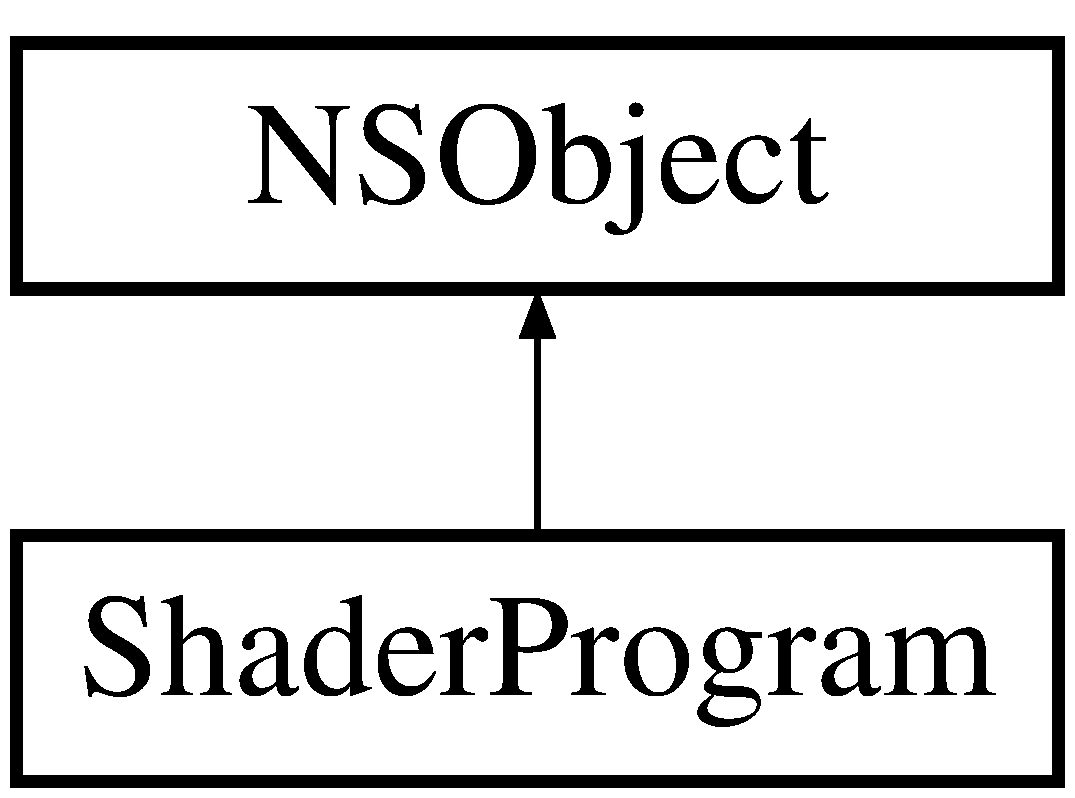
\includegraphics[height=2.000000cm]{interface_shader_program}
\end{center}
\end{figure}
\subsection*{Instance Methods}
\begin{DoxyCompactItemize}
\item 
(G\+Luint) -\/ \hyperlink{interface_shader_program_a20c6a3edaabcdd846f1ede37bba77cc6}{get\+Program\+Id}
\item 
(void) -\/ \hyperlink{interface_shader_program_a29d4892a17f1ed3aab31392d562eb46d}{set\+Program\+Id\+:}
\item 
(G\+Luint) -\/ \hyperlink{interface_shader_program_a31c59e1150529b7f91e083741eca49aa}{get\+Vertex\+Shader\+Id}
\item 
(void) -\/ \hyperlink{interface_shader_program_a0e68cf1773e4c63c085ad1edf7a82d80}{set\+Vertex\+Shader\+Id\+:}
\item 
(G\+Luint) -\/ \hyperlink{interface_shader_program_aee0c71ef492745e56530b0ce64d275c7}{get\+Fragment\+Shader\+Id}
\item 
(void) -\/ \hyperlink{interface_shader_program_ab368985d26b2947b692625069a916b45}{set\+Fragment\+Shader\+Id\+:}
\end{DoxyCompactItemize}


\subsection{Method Documentation}
\index{Shader\+Program@{Shader\+Program}!get\+Fragment\+Shader\+Id@{get\+Fragment\+Shader\+Id}}
\index{get\+Fragment\+Shader\+Id@{get\+Fragment\+Shader\+Id}!Shader\+Program@{Shader\+Program}}
\subsubsection[{\texorpdfstring{get\+Fragment\+Shader\+Id()}{getFragmentShaderId()}}]{\setlength{\rightskip}{0pt plus 5cm}-\/ (G\+Luint) get\+Fragment\+Shader\+Id 
\begin{DoxyParamCaption}
{}
\end{DoxyParamCaption}
}\hypertarget{interface_shader_program_aee0c71ef492745e56530b0ce64d275c7}{}\label{interface_shader_program_aee0c71ef492745e56530b0ce64d275c7}
\begin{DoxyReturn}{Returns}
the fragment\+Shader\+Id 
\end{DoxyReturn}
\index{Shader\+Program@{Shader\+Program}!get\+Program\+Id@{get\+Program\+Id}}
\index{get\+Program\+Id@{get\+Program\+Id}!Shader\+Program@{Shader\+Program}}
\subsubsection[{\texorpdfstring{get\+Program\+Id()}{getProgramId()}}]{\setlength{\rightskip}{0pt plus 5cm}-\/ (G\+Luint) get\+Program\+Id 
\begin{DoxyParamCaption}
{}
\end{DoxyParamCaption}
}\hypertarget{interface_shader_program_a20c6a3edaabcdd846f1ede37bba77cc6}{}\label{interface_shader_program_a20c6a3edaabcdd846f1ede37bba77cc6}
\begin{DoxyReturn}{Returns}
the program\+Id 
\end{DoxyReturn}
\index{Shader\+Program@{Shader\+Program}!get\+Vertex\+Shader\+Id@{get\+Vertex\+Shader\+Id}}
\index{get\+Vertex\+Shader\+Id@{get\+Vertex\+Shader\+Id}!Shader\+Program@{Shader\+Program}}
\subsubsection[{\texorpdfstring{get\+Vertex\+Shader\+Id()}{getVertexShaderId()}}]{\setlength{\rightskip}{0pt plus 5cm}-\/ (G\+Luint) get\+Vertex\+Shader\+Id 
\begin{DoxyParamCaption}
{}
\end{DoxyParamCaption}
}\hypertarget{interface_shader_program_a31c59e1150529b7f91e083741eca49aa}{}\label{interface_shader_program_a31c59e1150529b7f91e083741eca49aa}
\begin{DoxyReturn}{Returns}
the vertex\+Shader\+Id 
\end{DoxyReturn}
\index{Shader\+Program@{Shader\+Program}!set\+Fragment\+Shader\+Id\+:@{set\+Fragment\+Shader\+Id\+:}}
\index{set\+Fragment\+Shader\+Id\+:@{set\+Fragment\+Shader\+Id\+:}!Shader\+Program@{Shader\+Program}}
\subsubsection[{\texorpdfstring{set\+Fragment\+Shader\+Id\+:(\+G\+Luint fragment\+Shader\+Id)}{setFragmentShaderId:(GLuint fragmentShaderId)}}]{\setlength{\rightskip}{0pt plus 5cm}-\/ (void) set\+Fragment\+Shader\+Id\+: 
\begin{DoxyParamCaption}
\item[{(G\+Luint)}]{fragment\+Shader\+Id}
\end{DoxyParamCaption}
}\hypertarget{interface_shader_program_ab368985d26b2947b692625069a916b45}{}\label{interface_shader_program_ab368985d26b2947b692625069a916b45}

\begin{DoxyParams}{Parameters}
{\em fragment\+Shader\+Id} & the fragment\+Shader\+Id to set \\
\hline
\end{DoxyParams}
\index{Shader\+Program@{Shader\+Program}!set\+Program\+Id\+:@{set\+Program\+Id\+:}}
\index{set\+Program\+Id\+:@{set\+Program\+Id\+:}!Shader\+Program@{Shader\+Program}}
\subsubsection[{\texorpdfstring{set\+Program\+Id\+:(\+G\+Luint program\+Id)}{setProgramId:(GLuint programId)}}]{\setlength{\rightskip}{0pt plus 5cm}-\/ (void) set\+Program\+Id\+: 
\begin{DoxyParamCaption}
\item[{(G\+Luint)}]{program\+Id}
\end{DoxyParamCaption}
}\hypertarget{interface_shader_program_a29d4892a17f1ed3aab31392d562eb46d}{}\label{interface_shader_program_a29d4892a17f1ed3aab31392d562eb46d}

\begin{DoxyParams}{Parameters}
{\em program\+Id} & the program\+Id to set \\
\hline
\end{DoxyParams}
\index{Shader\+Program@{Shader\+Program}!set\+Vertex\+Shader\+Id\+:@{set\+Vertex\+Shader\+Id\+:}}
\index{set\+Vertex\+Shader\+Id\+:@{set\+Vertex\+Shader\+Id\+:}!Shader\+Program@{Shader\+Program}}
\subsubsection[{\texorpdfstring{set\+Vertex\+Shader\+Id\+:(\+G\+Luint vertex\+Shader\+Id)}{setVertexShaderId:(GLuint vertexShaderId)}}]{\setlength{\rightskip}{0pt plus 5cm}-\/ (void) set\+Vertex\+Shader\+Id\+: 
\begin{DoxyParamCaption}
\item[{(G\+Luint)}]{vertex\+Shader\+Id}
\end{DoxyParamCaption}
}\hypertarget{interface_shader_program_a0e68cf1773e4c63c085ad1edf7a82d80}{}\label{interface_shader_program_a0e68cf1773e4c63c085ad1edf7a82d80}

\begin{DoxyParams}{Parameters}
{\em vertex\+Shader\+Id} & the vertex\+Shader\+Id to set \\
\hline
\end{DoxyParams}


The documentation for this class was generated from the following files\+:\begin{DoxyCompactItemize}
\item 
Game\+Engine/\+Commons/Shader\+Program.\+h\item 
Game\+Engine/\+Commons/Shader\+Program.\+m\end{DoxyCompactItemize}

\hypertarget{interface_sky_box}{}\section{Sky\+Box Class Reference}
\label{interface_sky_box}\index{Sky\+Box@{Sky\+Box}}


{\ttfamily \#import $<$Sky\+Box.\+h$>$}

Inheritance diagram for Sky\+Box\+:\begin{figure}[H]
\begin{center}
\leavevmode
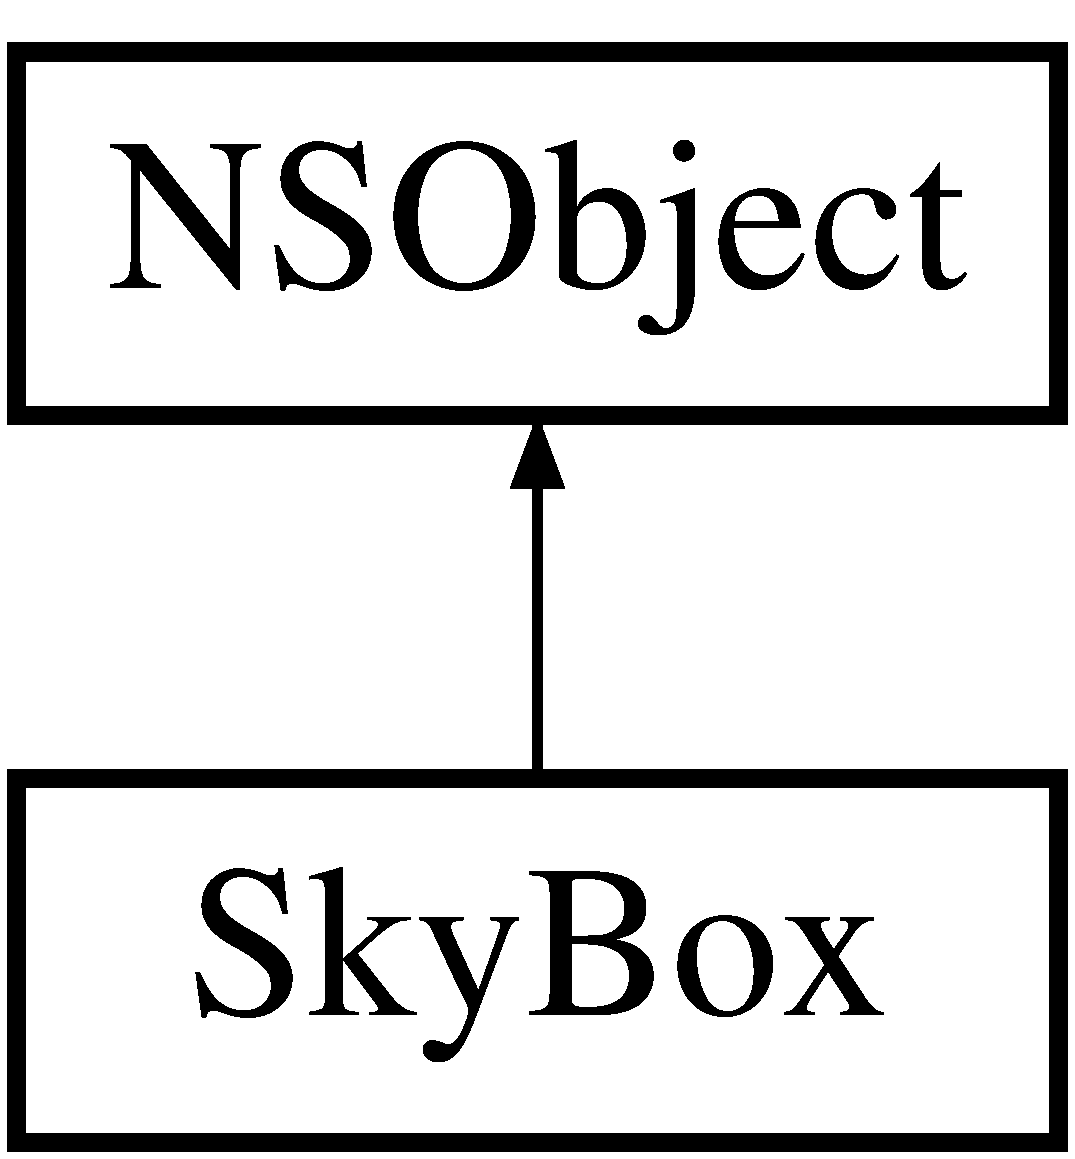
\includegraphics[height=2.000000cm]{interface_sky_box}
\end{center}
\end{figure}
\subsection*{Instance Methods}
\begin{DoxyCompactItemize}
\item 
(id) -\/ \hyperlink{interface_sky_box_af3c3b24551b18d6215fe5d5081d4a311}{init\+::}
\end{DoxyCompactItemize}
\subsection*{Properties}
\begin{DoxyCompactItemize}
\item 
\hyperlink{interface_raw_model}{Raw\+Model} $\ast$ \hyperlink{interface_sky_box_a7fb03172216b3054105f3b04c8e25d59}{model}
\item 
int \hyperlink{interface_sky_box_afe0139e67627fa13a821e58c0e7b746c}{texture\+Id}
\end{DoxyCompactItemize}


\subsection{Detailed Description}
Represents a box with sky textures 

\subsection{Method Documentation}
\index{Sky\+Box@{Sky\+Box}!init\+::@{init\+::}}
\index{init\+::@{init\+::}!Sky\+Box@{Sky\+Box}}
\subsubsection[{\texorpdfstring{init\+::(int a\+Texture\+Id,[] Raw\+Model $\ast$a\+Model)}{init::(int aTextureId,[] RawModel *aModel)}}]{\setlength{\rightskip}{0pt plus 5cm}-\/ (id) init\+: 
\begin{DoxyParamCaption}
\item[{(int)}]{a\+Texture\+Id}
\item[{:({\bf Raw\+Model}$\ast$)}]{a\+Model}
\end{DoxyParamCaption}
}\hypertarget{interface_sky_box_af3c3b24551b18d6215fe5d5081d4a311}{}\label{interface_sky_box_af3c3b24551b18d6215fe5d5081d4a311}
The initiator of the sky\+Box


\begin{DoxyParams}{Parameters}
{\em a\+Texture} & the Identifier of the texture of the sky \\
\hline
{\em a\+Model} & The model of the sky box \\
\hline
\end{DoxyParams}


\subsection{Property Documentation}
\index{Sky\+Box@{Sky\+Box}!model@{model}}
\index{model@{model}!Sky\+Box@{Sky\+Box}}
\subsubsection[{\texorpdfstring{model}{model}}]{\setlength{\rightskip}{0pt plus 5cm}-\/ ({\bf Raw\+Model}$\ast$) model\hspace{0.3cm}{\ttfamily [read]}, {\ttfamily [atomic]}, {\ttfamily [assign]}}\hypertarget{interface_sky_box_a7fb03172216b3054105f3b04c8e25d59}{}\label{interface_sky_box_a7fb03172216b3054105f3b04c8e25d59}
\hyperlink{interface_raw_model}{Raw\+Model} of the sky\+Box \index{Sky\+Box@{Sky\+Box}!texture\+Id@{texture\+Id}}
\index{texture\+Id@{texture\+Id}!Sky\+Box@{Sky\+Box}}
\subsubsection[{\texorpdfstring{texture\+Id}{textureId}}]{\setlength{\rightskip}{0pt plus 5cm}-\/ (int) texture\+Id\hspace{0.3cm}{\ttfamily [read]}, {\ttfamily [atomic]}, {\ttfamily [assign]}}\hypertarget{interface_sky_box_afe0139e67627fa13a821e58c0e7b746c}{}\label{interface_sky_box_afe0139e67627fa13a821e58c0e7b746c}
The identifier of the sky box cubic texture 

The documentation for this class was generated from the following files\+:\begin{DoxyCompactItemize}
\item 
Game\+Engine/\+Models/Sky\+Box.\+h\item 
Game\+Engine/\+Models/Sky\+Box.\+m\end{DoxyCompactItemize}

\hypertarget{interface_sky_box_shape}{}\section{Sky\+Box\+Shape Class Reference}
\label{interface_sky_box_shape}\index{Sky\+Box\+Shape@{Sky\+Box\+Shape}}
Inheritance diagram for Sky\+Box\+Shape\+:\begin{figure}[H]
\begin{center}
\leavevmode
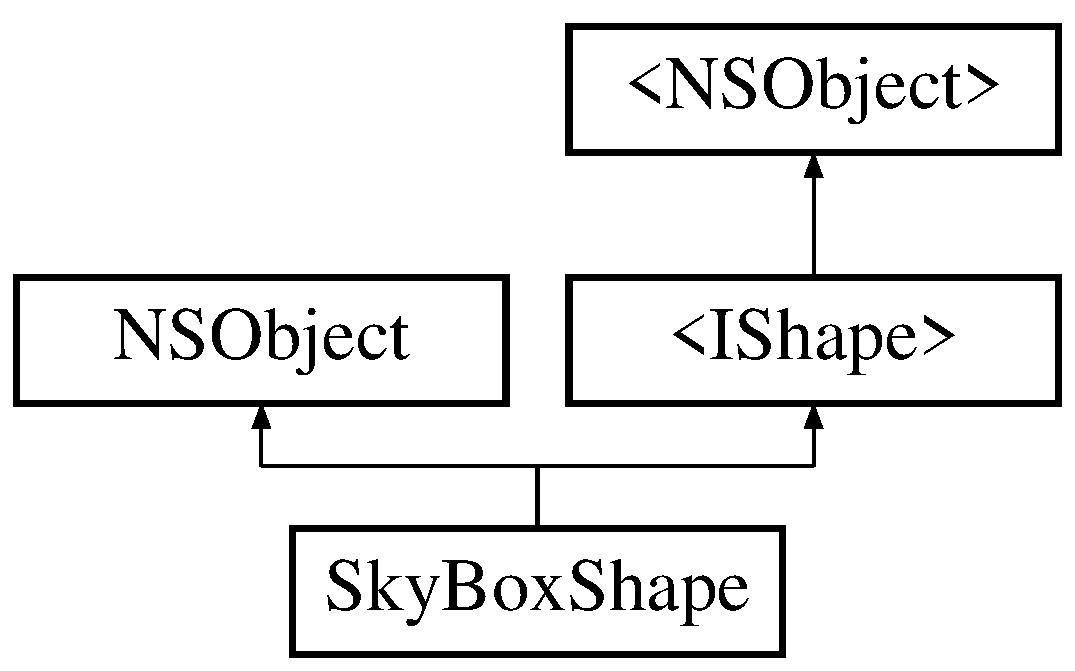
\includegraphics[height=3.000000cm]{interface_sky_box_shape}
\end{center}
\end{figure}
\subsection*{Instance Methods}
\begin{DoxyCompactItemize}
\item 
(id) -\/ \hyperlink{interface_sky_box_shape_a90cd48180de4a0776299354dedd412af}{init}
\end{DoxyCompactItemize}


\subsection{Detailed Description}
Represents the sky box in the 3D world 

\subsection{Method Documentation}
\index{Sky\+Box\+Shape@{Sky\+Box\+Shape}!init@{init}}
\index{init@{init}!Sky\+Box\+Shape@{Sky\+Box\+Shape}}
\subsubsection[{\texorpdfstring{init()}{init()}}]{\setlength{\rightskip}{0pt plus 5cm}-\/ (id) init 
\begin{DoxyParamCaption}
{}
\end{DoxyParamCaption}
}\hypertarget{interface_sky_box_shape_a90cd48180de4a0776299354dedd412af}{}\label{interface_sky_box_shape_a90cd48180de4a0776299354dedd412af}
Initiator of the sky box shape 

The documentation for this class was generated from the following files\+:\begin{DoxyCompactItemize}
\item 
Game\+Engine/\+Models/Sky\+Box\+Shape.\+h\item 
Game\+Engine/\+Models/Sky\+Box\+Shape.\+m\end{DoxyCompactItemize}

\hypertarget{interface_terrain}{}\section{Terrain Class Reference}
\label{interface_terrain}\index{Terrain@{Terrain}}


{\ttfamily \#import $<$Terrain.\+h$>$}

Inheritance diagram for Terrain\+:\begin{figure}[H]
\begin{center}
\leavevmode
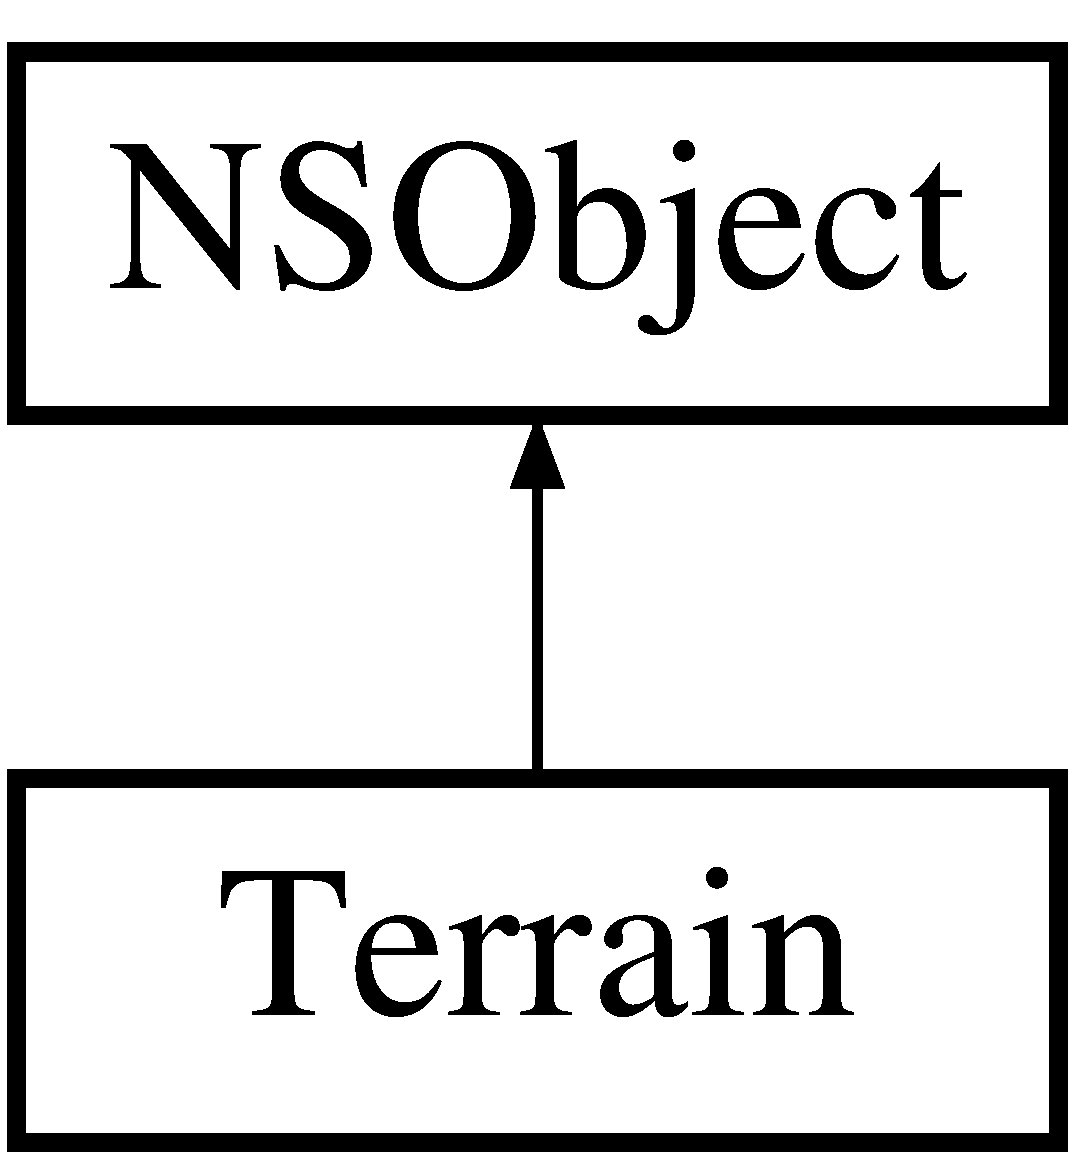
\includegraphics[height=2.000000cm]{interface_terrain}
\end{center}
\end{figure}
\subsection*{Properties}
\begin{DoxyCompactItemize}
\item 
float \hyperlink{interface_terrain_a47761d42d9c6a4ffc7df3a5bf93b7ef2}{x}
\item 
float \hyperlink{interface_terrain_a6f91dd10a551c69436bee85b674bbdc4}{y}
\item 
float \hyperlink{interface_terrain_abf8b4e04a0571cd394dbef7e2b0f06ac}{z}
\item 
\hyperlink{interface_raw_model}{Raw\+Model} $\ast$ \hyperlink{interface_terrain_aeb3387c4f77d2b3403f8ad5e427018ac}{model}
\end{DoxyCompactItemize}


\subsection{Detailed Description}
The model to the terrain entity 

\subsection{Property Documentation}
\index{Terrain@{Terrain}!model@{model}}
\index{model@{model}!Terrain@{Terrain}}
\subsubsection[{\texorpdfstring{model}{model}}]{\setlength{\rightskip}{0pt plus 5cm}-\/ ({\bf Raw\+Model}$\ast$) model\hspace{0.3cm}{\ttfamily [read]}, {\ttfamily [atomic]}, {\ttfamily [assign]}}\hypertarget{interface_terrain_aeb3387c4f77d2b3403f8ad5e427018ac}{}\label{interface_terrain_aeb3387c4f77d2b3403f8ad5e427018ac}
\hyperlink{interface_raw_model}{Raw\+Model} of the terrain \index{Terrain@{Terrain}!x@{x}}
\index{x@{x}!Terrain@{Terrain}}
\subsubsection[{\texorpdfstring{x}{x}}]{\setlength{\rightskip}{0pt plus 5cm}-\/ (float) x\hspace{0.3cm}{\ttfamily [read]}, {\ttfamily [atomic]}, {\ttfamily [assign]}}\hypertarget{interface_terrain_a47761d42d9c6a4ffc7df3a5bf93b7ef2}{}\label{interface_terrain_a47761d42d9c6a4ffc7df3a5bf93b7ef2}
Position of the terrain in the x-\/axle \index{Terrain@{Terrain}!y@{y}}
\index{y@{y}!Terrain@{Terrain}}
\subsubsection[{\texorpdfstring{y}{y}}]{\setlength{\rightskip}{0pt plus 5cm}-\/ (float) y\hspace{0.3cm}{\ttfamily [read]}, {\ttfamily [atomic]}, {\ttfamily [assign]}}\hypertarget{interface_terrain_a6f91dd10a551c69436bee85b674bbdc4}{}\label{interface_terrain_a6f91dd10a551c69436bee85b674bbdc4}
Position of the terrain in the y-\/axle \index{Terrain@{Terrain}!z@{z}}
\index{z@{z}!Terrain@{Terrain}}
\subsubsection[{\texorpdfstring{z}{z}}]{\setlength{\rightskip}{0pt plus 5cm}-\/ (float) z\hspace{0.3cm}{\ttfamily [read]}, {\ttfamily [atomic]}, {\ttfamily [assign]}}\hypertarget{interface_terrain_abf8b4e04a0571cd394dbef7e2b0f06ac}{}\label{interface_terrain_abf8b4e04a0571cd394dbef7e2b0f06ac}
Position of the terrain in the z-\/axle 

The documentation for this class was generated from the following file\+:\begin{DoxyCompactItemize}
\item 
Game\+Engine/\+Models/Terrain.\+h\end{DoxyCompactItemize}

\hypertarget{interface_terrain_shape}{}\section{Terrain\+Shape Class Reference}
\label{interface_terrain_shape}\index{Terrain\+Shape@{Terrain\+Shape}}


{\ttfamily \#import $<$Terrain\+Shape.\+h$>$}

Inheritance diagram for Terrain\+Shape\+:\begin{figure}[H]
\begin{center}
\leavevmode
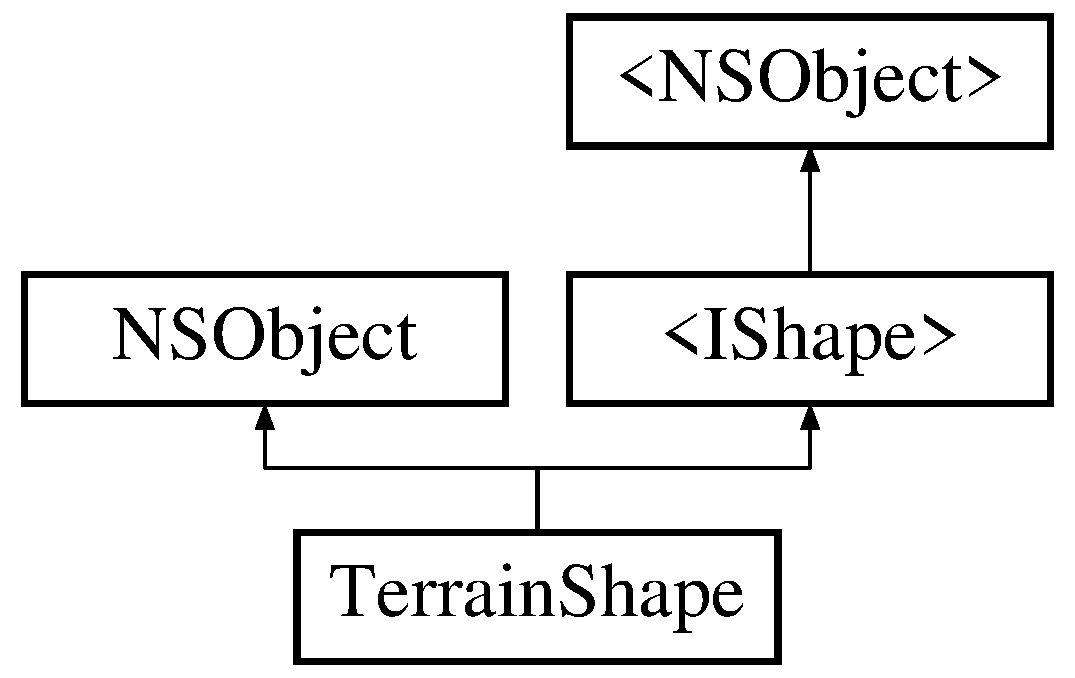
\includegraphics[height=3.000000cm]{interface_terrain_shape}
\end{center}
\end{figure}
\subsection*{Instance Methods}
\begin{DoxyCompactItemize}
\item 
(id) -\/ \hyperlink{interface_terrain_shape_ac193c05fd7c19b5c63dcd2900e624ff5}{init}
\end{DoxyCompactItemize}


\subsection{Detailed Description}
Represents one terrain in the 3D world 

\subsection{Method Documentation}
\index{Terrain\+Shape@{Terrain\+Shape}!init@{init}}
\index{init@{init}!Terrain\+Shape@{Terrain\+Shape}}
\subsubsection[{\texorpdfstring{init()}{init()}}]{\setlength{\rightskip}{0pt plus 5cm}-\/ (id) init 
\begin{DoxyParamCaption}
{}
\end{DoxyParamCaption}
}\hypertarget{interface_terrain_shape_ac193c05fd7c19b5c63dcd2900e624ff5}{}\label{interface_terrain_shape_ac193c05fd7c19b5c63dcd2900e624ff5}
Initiator of the terrain shape 

The documentation for this class was generated from the following files\+:\begin{DoxyCompactItemize}
\item 
Game\+Engine/\+Models/Terrain\+Shape.\+h\item 
Game\+Engine/\+Models/Terrain\+Shape.\+m\end{DoxyCompactItemize}

\hypertarget{interface_terrain_textures_pack}{}\section{Terrain\+Textures\+Pack Class Reference}
\label{interface_terrain_textures_pack}\index{Terrain\+Textures\+Pack@{Terrain\+Textures\+Pack}}


{\ttfamily \#import $<$Terrain\+Textures\+Pack.\+h$>$}

Inheritance diagram for Terrain\+Textures\+Pack\+:\begin{figure}[H]
\begin{center}
\leavevmode
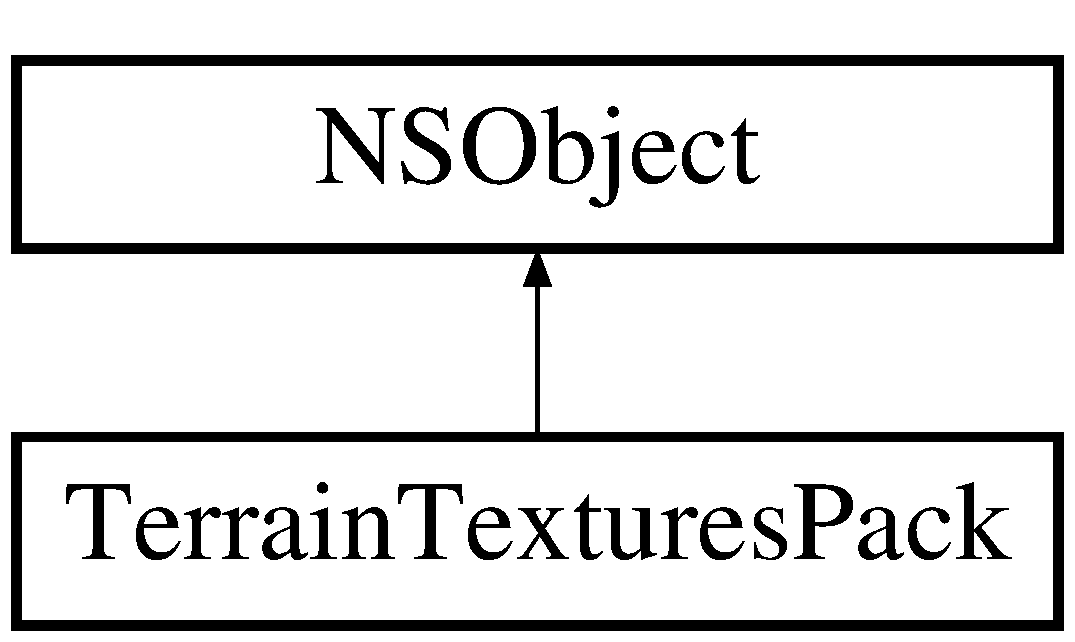
\includegraphics[height=2.000000cm]{interface_terrain_textures_pack}
\end{center}
\end{figure}
\subsection*{Properties}
\begin{DoxyCompactItemize}
\item 
int \hyperlink{interface_terrain_textures_pack_aaff06a2e112ae5f534b3bdd4804e7659}{weight\+Map\+Texture\+Id}
\item 
int \hyperlink{interface_terrain_textures_pack_aaf22ea7a7c4b7a9bea89865b86472cd8}{background\+Texture\+Id}
\item 
int \hyperlink{interface_terrain_textures_pack_a293f99431d498c17bdf6f20bb9842a8e}{mud\+Texture\+Id}
\item 
int \hyperlink{interface_terrain_textures_pack_aeb36cd29e8a709d1c334cf6b7422bfa1}{grass\+Texture\+Id}
\item 
int \hyperlink{interface_terrain_textures_pack_af893c59088e91ded731cb431df095a64}{path\+Texture\+Id}
\end{DoxyCompactItemize}


\subsection{Detailed Description}
Contains the identifiers to the several textures of a terrain 

\subsection{Property Documentation}
\index{Terrain\+Textures\+Pack@{Terrain\+Textures\+Pack}!background\+Texture\+Id@{background\+Texture\+Id}}
\index{background\+Texture\+Id@{background\+Texture\+Id}!Terrain\+Textures\+Pack@{Terrain\+Textures\+Pack}}
\subsubsection[{\texorpdfstring{background\+Texture\+Id}{backgroundTextureId}}]{\setlength{\rightskip}{0pt plus 5cm}-\/ (int) background\+Texture\+Id\hspace{0.3cm}{\ttfamily [read]}, {\ttfamily [write]}, {\ttfamily [atomic]}}\hypertarget{interface_terrain_textures_pack_aaf22ea7a7c4b7a9bea89865b86472cd8}{}\label{interface_terrain_textures_pack_aaf22ea7a7c4b7a9bea89865b86472cd8}
The identifier of the background texture \index{Terrain\+Textures\+Pack@{Terrain\+Textures\+Pack}!grass\+Texture\+Id@{grass\+Texture\+Id}}
\index{grass\+Texture\+Id@{grass\+Texture\+Id}!Terrain\+Textures\+Pack@{Terrain\+Textures\+Pack}}
\subsubsection[{\texorpdfstring{grass\+Texture\+Id}{grassTextureId}}]{\setlength{\rightskip}{0pt plus 5cm}-\/ (int) grass\+Texture\+Id\hspace{0.3cm}{\ttfamily [read]}, {\ttfamily [write]}, {\ttfamily [atomic]}}\hypertarget{interface_terrain_textures_pack_aeb36cd29e8a709d1c334cf6b7422bfa1}{}\label{interface_terrain_textures_pack_aeb36cd29e8a709d1c334cf6b7422bfa1}
Identifier of the grass texture \index{Terrain\+Textures\+Pack@{Terrain\+Textures\+Pack}!mud\+Texture\+Id@{mud\+Texture\+Id}}
\index{mud\+Texture\+Id@{mud\+Texture\+Id}!Terrain\+Textures\+Pack@{Terrain\+Textures\+Pack}}
\subsubsection[{\texorpdfstring{mud\+Texture\+Id}{mudTextureId}}]{\setlength{\rightskip}{0pt plus 5cm}-\/ (int) mud\+Texture\+Id\hspace{0.3cm}{\ttfamily [read]}, {\ttfamily [write]}, {\ttfamily [atomic]}}\hypertarget{interface_terrain_textures_pack_a293f99431d498c17bdf6f20bb9842a8e}{}\label{interface_terrain_textures_pack_a293f99431d498c17bdf6f20bb9842a8e}
Identifier of the mud texture \index{Terrain\+Textures\+Pack@{Terrain\+Textures\+Pack}!path\+Texture\+Id@{path\+Texture\+Id}}
\index{path\+Texture\+Id@{path\+Texture\+Id}!Terrain\+Textures\+Pack@{Terrain\+Textures\+Pack}}
\subsubsection[{\texorpdfstring{path\+Texture\+Id}{pathTextureId}}]{\setlength{\rightskip}{0pt plus 5cm}-\/ (int) path\+Texture\+Id\hspace{0.3cm}{\ttfamily [read]}, {\ttfamily [write]}, {\ttfamily [atomic]}}\hypertarget{interface_terrain_textures_pack_af893c59088e91ded731cb431df095a64}{}\label{interface_terrain_textures_pack_af893c59088e91ded731cb431df095a64}
Identifier of the path texture \index{Terrain\+Textures\+Pack@{Terrain\+Textures\+Pack}!weight\+Map\+Texture\+Id@{weight\+Map\+Texture\+Id}}
\index{weight\+Map\+Texture\+Id@{weight\+Map\+Texture\+Id}!Terrain\+Textures\+Pack@{Terrain\+Textures\+Pack}}
\subsubsection[{\texorpdfstring{weight\+Map\+Texture\+Id}{weightMapTextureId}}]{\setlength{\rightskip}{0pt plus 5cm}-\/ (int) weight\+Map\+Texture\+Id\hspace{0.3cm}{\ttfamily [read]}, {\ttfamily [write]}, {\ttfamily [atomic]}}\hypertarget{interface_terrain_textures_pack_aaff06a2e112ae5f534b3bdd4804e7659}{}\label{interface_terrain_textures_pack_aaff06a2e112ae5f534b3bdd4804e7659}
The identifier of the weight map texture 

The documentation for this class was generated from the following file\+:\begin{DoxyCompactItemize}
\item 
Game\+Engine/\+Textures/Terrain\+Textures\+Pack.\+h\end{DoxyCompactItemize}

\hypertarget{interface_textured_model}{}\section{Textured\+Model Class Reference}
\label{interface_textured_model}\index{Textured\+Model@{Textured\+Model}}


{\ttfamily \#import $<$Textured\+Model.\+h$>$}

Inheritance diagram for Textured\+Model\+:\begin{figure}[H]
\begin{center}
\leavevmode
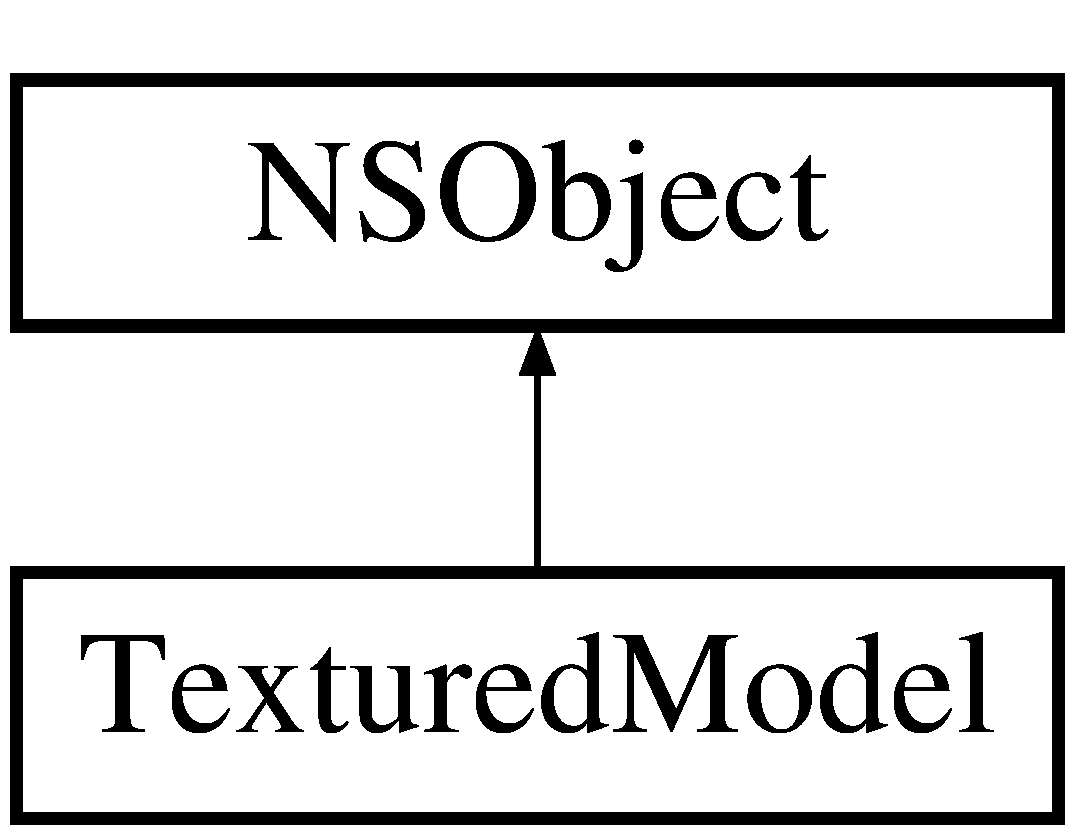
\includegraphics[height=2.000000cm]{interface_textured_model}
\end{center}
\end{figure}
\subsection*{Instance Methods}
\begin{DoxyCompactItemize}
\item 
(\hyperlink{interface_textured_model_aca9eab5290f81898de99b46078419ebc}{id}) -\/ \hyperlink{interface_textured_model_a0beb4248998bf716095b537fce368336}{init\+::::}
\item 
(\hyperlink{interface_textured_model_aca9eab5290f81898de99b46078419ebc}{id}) -\/ \hyperlink{interface_textured_model_aeef3037569cd0cd46a06023070fa4854}{init\+::}
\end{DoxyCompactItemize}
\subsection*{Properties}
\begin{DoxyCompactItemize}
\item 
long \hyperlink{interface_textured_model_aca9eab5290f81898de99b46078419ebc}{id}
\item 
\hyperlink{interface_raw_model}{Raw\+Model} $\ast$ \hyperlink{interface_textured_model_a502115a1985353177ee79ee41bf5f88f}{raw\+Model}
\item 
\hyperlink{interface_model_texture}{Model\+Texture} $\ast$ \hyperlink{interface_textured_model_a4044c19645d8a4dbb6bb1e7c0fe8d5e9}{texture}
\item 
B\+O\+OL \hyperlink{interface_textured_model_a025325456b8589e41a1d514a5424f0fa}{has\+Transparency}
\item 
B\+O\+OL \hyperlink{interface_textured_model_a04689af3a31961d1f4fcf058e264c3c8}{normals\+Pointing\+Up}
\end{DoxyCompactItemize}


\subsection{Detailed Description}
Wrapper that besides of have the raw model also has the texture to put in the model 

\subsection{Method Documentation}
\index{Textured\+Model@{Textured\+Model}!init\+::@{init\+::}}
\index{init\+::@{init\+::}!Textured\+Model@{Textured\+Model}}
\subsubsection[{\texorpdfstring{init\+::(\+Raw\+Model $\ast$a\+Raw\+Model,[] Model\+Texture $\ast$texture)}{init::(RawModel *aRawModel,[] ModelTexture *texture)}}]{\setlength{\rightskip}{0pt plus 5cm}-\/ ({\bf id}) init\+: 
\begin{DoxyParamCaption}
\item[{({\bf Raw\+Model}$\ast$)}]{a\+Raw\+Model}
\item[{:({\bf Model\+Texture}$\ast$)}]{a\+Texture}
\end{DoxyParamCaption}
}\hypertarget{interface_textured_model_aeef3037569cd0cd46a06023070fa4854}{}\label{interface_textured_model_aeef3037569cd0cd46a06023070fa4854}
Initiator of the textured model 
\begin{DoxyParams}{Parameters}
{\em raw\+Model} & Raw model of the entity \\
\hline
{\em texture} & Reference to the texture of the entity\\
\hline
\end{DoxyParams}
Initiator of the textured model 
\begin{DoxyParams}{Parameters}
{\em a\+Raw\+Model} & Raw model of the entity \\
\hline
{\em a\+Texture} & Reference to the texture of the entity \\
\hline
\end{DoxyParams}
\index{Textured\+Model@{Textured\+Model}!init\+::::@{init\+::::}}
\index{init\+::::@{init\+::::}!Textured\+Model@{Textured\+Model}}
\subsubsection[{\texorpdfstring{init\+::::(\+Raw\+Model $\ast$a\+Raw\+Model,[] Model\+Texture $\ast$a\+Texture,[] bool a\+Has\+Transparency,[] bool a\+Normals\+Pointing\+Up)}{init::::(RawModel *aRawModel,[] ModelTexture *aTexture,[] bool aHasTransparency,[] bool aNormalsPointingUp)}}]{\setlength{\rightskip}{0pt plus 5cm}-\/ ({\bf id}) init\+: 
\begin{DoxyParamCaption}
\item[{({\bf Raw\+Model}$\ast$)}]{a\+Raw\+Model}
\item[{:({\bf Model\+Texture}$\ast$)}]{a\+Texture}
\item[{:(bool)}]{a\+Has\+Transparency}
\item[{:(bool)}]{a\+Normals\+Pointing\+Up}
\end{DoxyParamCaption}
}\hypertarget{interface_textured_model_a0beb4248998bf716095b537fce368336}{}\label{interface_textured_model_a0beb4248998bf716095b537fce368336}
Initiator of the textured model


\begin{DoxyParams}{Parameters}
{\em a\+Raw\+Model} & Raw model of the entity \\
\hline
{\em a\+Texture} & Reference to the texture of the entity \\
\hline
{\em a\+Has\+Transparency} & Indicates if the model has transparency or not not \\
\hline
{\em a\+Normals\+Pointing\+Up} & Indicates if the normals of the model should point up \\
\hline
\end{DoxyParams}


\subsection{Property Documentation}
\index{Textured\+Model@{Textured\+Model}!has\+Transparency@{has\+Transparency}}
\index{has\+Transparency@{has\+Transparency}!Textured\+Model@{Textured\+Model}}
\subsubsection[{\texorpdfstring{has\+Transparency}{hasTransparency}}]{\setlength{\rightskip}{0pt plus 5cm}-\/ (B\+O\+OL) has\+Transparency\hspace{0.3cm}{\ttfamily [read]}, {\ttfamily [atomic]}, {\ttfamily [assign]}}\hypertarget{interface_textured_model_a025325456b8589e41a1d514a5424f0fa}{}\label{interface_textured_model_a025325456b8589e41a1d514a5424f0fa}
Indicates if the model has transparency or not \index{Textured\+Model@{Textured\+Model}!id@{id}}
\index{id@{id}!Textured\+Model@{Textured\+Model}}
\subsubsection[{\texorpdfstring{id}{id}}]{\setlength{\rightskip}{0pt plus 5cm}-\/ (long) id\hspace{0.3cm}{\ttfamily [read]}, {\ttfamily [atomic]}, {\ttfamily [assign]}}\hypertarget{interface_textured_model_aca9eab5290f81898de99b46078419ebc}{}\label{interface_textured_model_aca9eab5290f81898de99b46078419ebc}
Identifier of the textured model \index{Textured\+Model@{Textured\+Model}!normals\+Pointing\+Up@{normals\+Pointing\+Up}}
\index{normals\+Pointing\+Up@{normals\+Pointing\+Up}!Textured\+Model@{Textured\+Model}}
\subsubsection[{\texorpdfstring{normals\+Pointing\+Up}{normalsPointingUp}}]{\setlength{\rightskip}{0pt plus 5cm}-\/ (B\+O\+OL) normals\+Pointing\+Up\hspace{0.3cm}{\ttfamily [read]}, {\ttfamily [write]}, {\ttfamily [atomic]}}\hypertarget{interface_textured_model_a04689af3a31961d1f4fcf058e264c3c8}{}\label{interface_textured_model_a04689af3a31961d1f4fcf058e264c3c8}
Indicate that all our normals of the object are going to point up (in the same direction \index{Textured\+Model@{Textured\+Model}!raw\+Model@{raw\+Model}}
\index{raw\+Model@{raw\+Model}!Textured\+Model@{Textured\+Model}}
\subsubsection[{\texorpdfstring{raw\+Model}{rawModel}}]{\setlength{\rightskip}{0pt plus 5cm}-\/ ({\bf Raw\+Model}$\ast$) raw\+Model\hspace{0.3cm}{\ttfamily [read]}, {\ttfamily [atomic]}, {\ttfamily [assign]}}\hypertarget{interface_textured_model_a502115a1985353177ee79ee41bf5f88f}{}\label{interface_textured_model_a502115a1985353177ee79ee41bf5f88f}
Raw model of the entity \index{Textured\+Model@{Textured\+Model}!texture@{texture}}
\index{texture@{texture}!Textured\+Model@{Textured\+Model}}
\subsubsection[{\texorpdfstring{texture}{texture}}]{\setlength{\rightskip}{0pt plus 5cm}-\/ ({\bf Model\+Texture}$\ast$) texture\hspace{0.3cm}{\ttfamily [read]}, {\ttfamily [atomic]}, {\ttfamily [assign]}}\hypertarget{interface_textured_model_a4044c19645d8a4dbb6bb1e7c0fe8d5e9}{}\label{interface_textured_model_a4044c19645d8a4dbb6bb1e7c0fe8d5e9}
Reference to the texture of the entity 

The documentation for this class was generated from the following files\+:\begin{DoxyCompactItemize}
\item 
Game\+Engine/\+Models/Textured\+Model.\+h\item 
Game\+Engine/\+Models/Textured\+Model.\+m\end{DoxyCompactItemize}

\hypertarget{interface_vector2f}{}\section{Vector2f Class Reference}
\label{interface_vector2f}\index{Vector2f@{Vector2f}}


{\ttfamily \#import $<$Vector2f.\+h$>$}

Inheritance diagram for Vector2f\+:\begin{figure}[H]
\begin{center}
\leavevmode
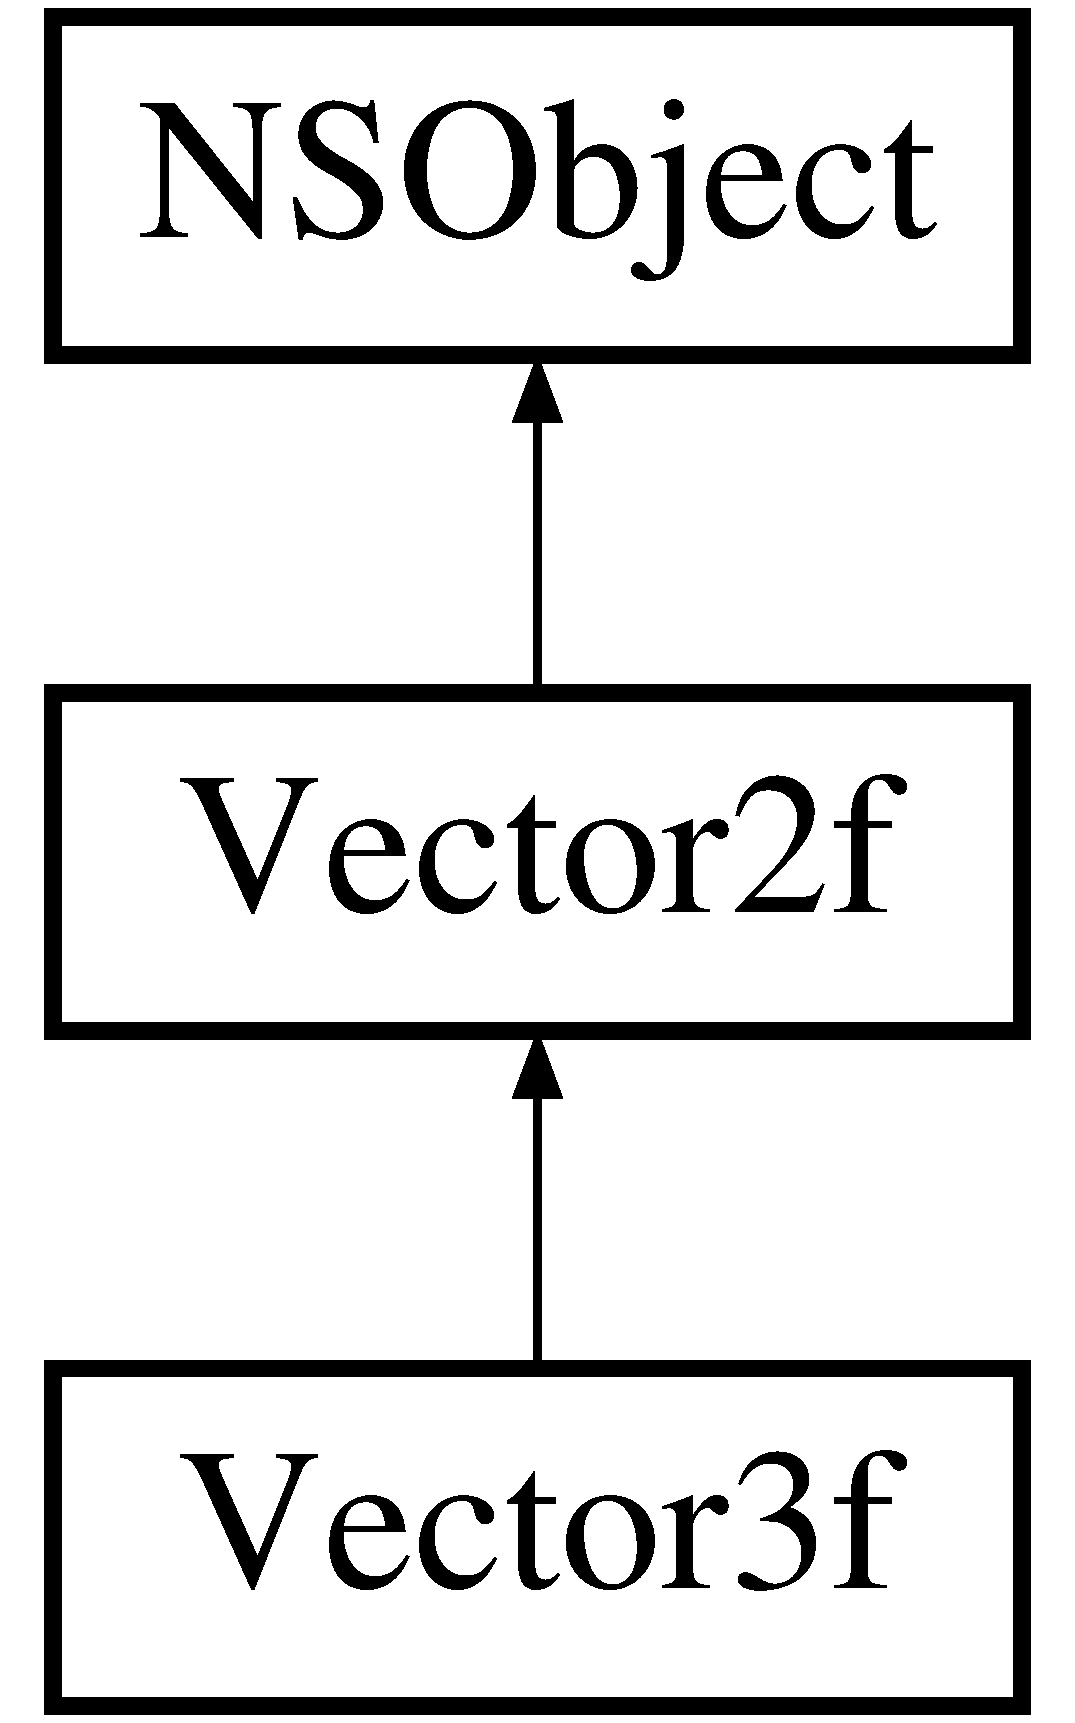
\includegraphics[height=3.000000cm]{interface_vector2f}
\end{center}
\end{figure}
\subsection*{Instance Methods}
\begin{DoxyCompactItemize}
\item 
(id) -\/ \hyperlink{interface_vector2f_aa75e63432eac74b4e29d6f926cd68fad}{init\+::}
\end{DoxyCompactItemize}
\subsection*{Properties}
\begin{DoxyCompactItemize}
\item 
float {\bfseries x}\hypertarget{interface_vector2f_add58d2378e3a3abdb76cf0ac51c9acfc}{}\label{interface_vector2f_add58d2378e3a3abdb76cf0ac51c9acfc}

\item 
float {\bfseries y}\hypertarget{interface_vector2f_a14874a72597fd358b15f8ba34b999c4d}{}\label{interface_vector2f_a14874a72597fd358b15f8ba34b999c4d}

\end{DoxyCompactItemize}


\subsection{Detailed Description}
Represents a 2D Vector with their x,y,z coordinates 

\subsection{Method Documentation}
\index{Vector2f@{Vector2f}!init\+::@{init\+::}}
\index{init\+::@{init\+::}!Vector2f@{Vector2f}}
\subsubsection[{\texorpdfstring{init\+::(float a\+X,[] float a\+Y)}{init::(float aX,[] float aY)}}]{\setlength{\rightskip}{0pt plus 5cm}-\/ (id) init\+: 
\begin{DoxyParamCaption}
\item[{(float)}]{aX}
\item[{:(float)}]{aY}
\end{DoxyParamCaption}
}\hypertarget{interface_vector2f_aa75e63432eac74b4e29d6f926cd68fad}{}\label{interface_vector2f_aa75e63432eac74b4e29d6f926cd68fad}
The initialize of the vector


\begin{DoxyParams}{Parameters}
{\em aX} & coordinate \\
\hline
{\em aY} & coordinate \\
\hline
\end{DoxyParams}


The documentation for this class was generated from the following files\+:\begin{DoxyCompactItemize}
\item 
Game\+Engine/\+Commons/Vector2f.\+h\item 
Game\+Engine/\+Commons/Vector2f.\+m\end{DoxyCompactItemize}

\hypertarget{interface_vector3f}{}\section{Vector3f Class Reference}
\label{interface_vector3f}\index{Vector3f@{Vector3f}}
Inheritance diagram for Vector3f\+:\begin{figure}[H]
\begin{center}
\leavevmode
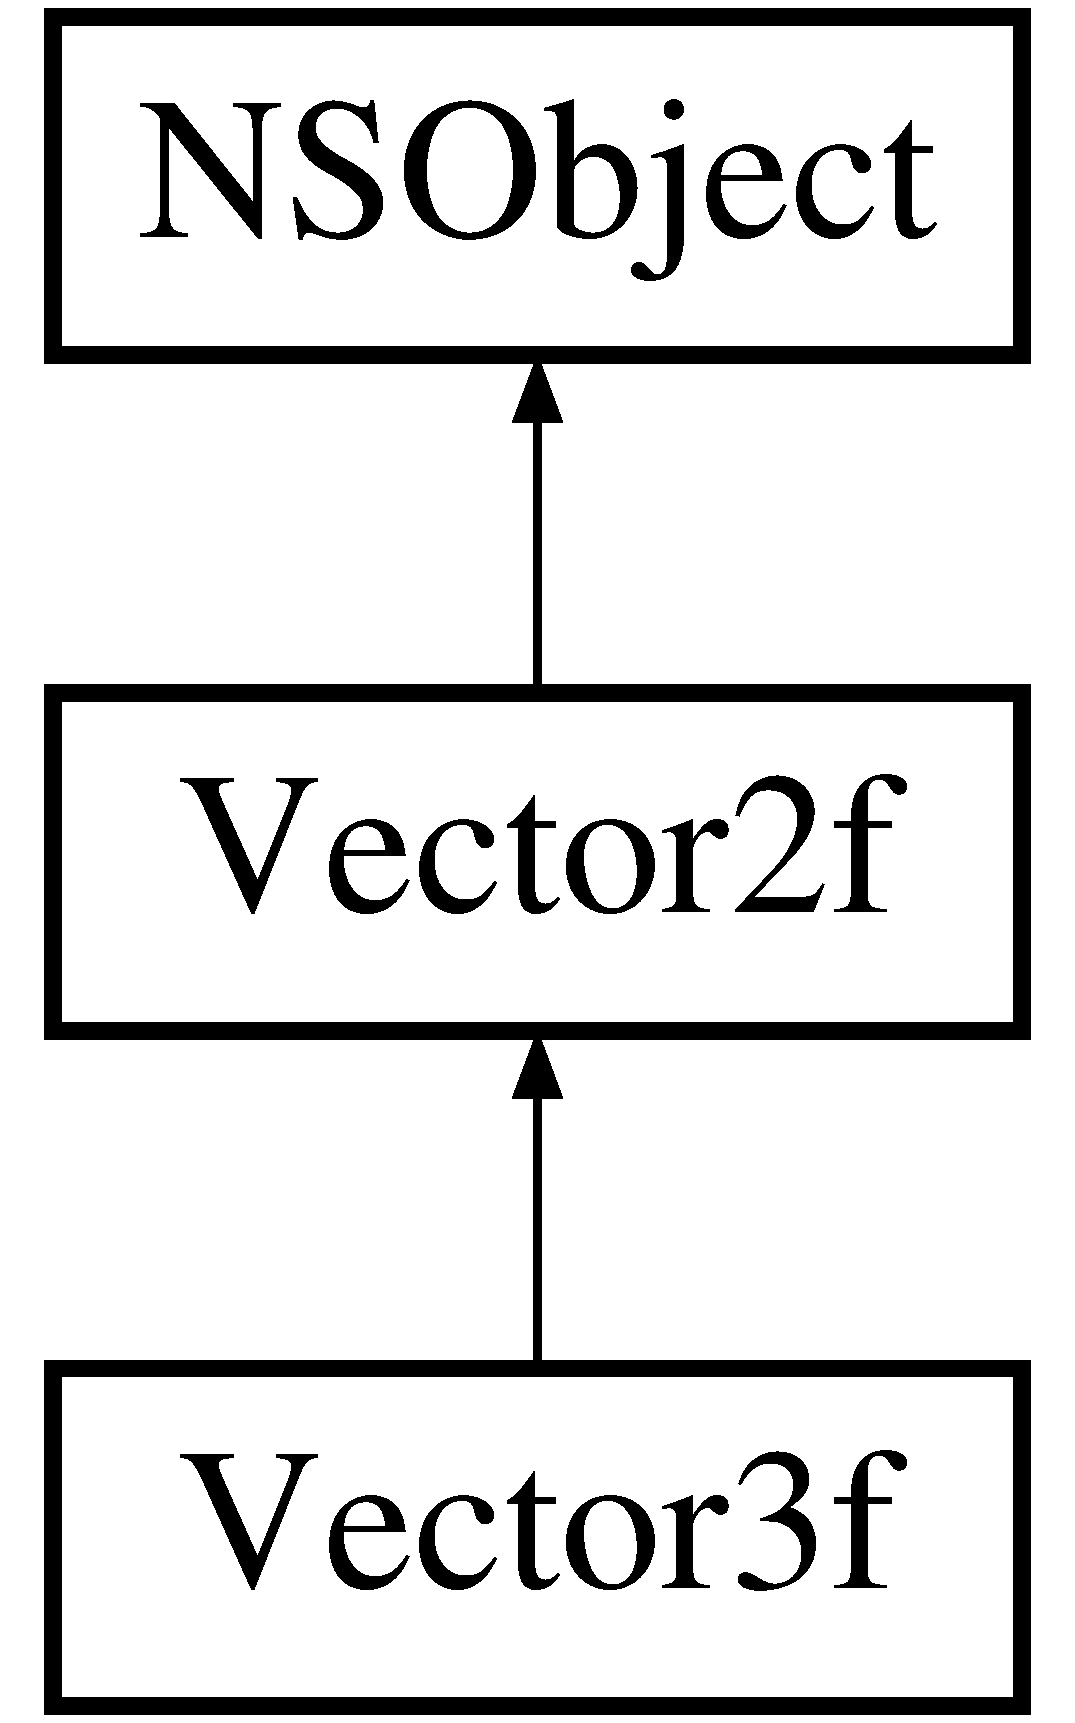
\includegraphics[height=3.000000cm]{interface_vector3f}
\end{center}
\end{figure}
\subsection*{Instance Methods}
\begin{DoxyCompactItemize}
\item 
(id) -\/ \hyperlink{interface_vector3f_a32eb5fdc556e0523987b17d8d0ab9fff}{init\+:::}
\end{DoxyCompactItemize}
\subsection*{Properties}
\begin{DoxyCompactItemize}
\item 
float {\bfseries z}\hypertarget{interface_vector3f_a470cff51eb6463672be518f5af4e26db}{}\label{interface_vector3f_a470cff51eb6463672be518f5af4e26db}

\end{DoxyCompactItemize}


\subsection{Method Documentation}
\index{Vector3f@{Vector3f}!init\+:::@{init\+:::}}
\index{init\+:::@{init\+:::}!Vector3f@{Vector3f}}
\subsubsection[{\texorpdfstring{init\+:::(float a\+X,[] float a\+Y,[] float a\+Z)}{init:::(float aX,[] float aY,[] float aZ)}}]{\setlength{\rightskip}{0pt plus 5cm}-\/ (id) init\+: 
\begin{DoxyParamCaption}
\item[{(float)}]{aX}
\item[{:(float)}]{aY}
\item[{:(float)}]{aZ}
\end{DoxyParamCaption}
}\hypertarget{interface_vector3f_a32eb5fdc556e0523987b17d8d0ab9fff}{}\label{interface_vector3f_a32eb5fdc556e0523987b17d8d0ab9fff}
The initialize of the vector


\begin{DoxyParams}{Parameters}
{\em aX} & coordinate \\
\hline
{\em aY} & coordinate \\
\hline
{\em aZ} & coordinate \\
\hline
\end{DoxyParams}


The documentation for this class was generated from the following files\+:\begin{DoxyCompactItemize}
\item 
Game\+Engine/\+Commons/Vector3f.\+h\item 
Game\+Engine/\+Commons/Vector3f.\+m\end{DoxyCompactItemize}

%--- End generated contents ---

% Index
\backmatter
\newpage
\phantomsection
\clearemptydoublepage
\addcontentsline{toc}{chapter}{Index}
\printindex

\end{document}
